%%%%%%%%%%%%%%%%%%%%%%%%%%%%%%%%%%%%%%%%%%%%%%%%%%%%%%%%%%
%
% Doctoral Thesis Template @ The University of Manchester
% LaTeX Chapter Template
% Version 1 (23/07/2020)
% Joe Crone
%
% This template is based on:
% The University of Manchester, Presentation of Thesis Policy
% Research Office Graduate Education Team
% June 2017
% http://www.regulations.manchester.ac.uk/pgr-presentation-theses/
%
%%%%%%%%%%%%%%%%%%%%%%%%%%%%%%%%%%%%%%%%%%%%%%%%%%%%%%%%%%
\documentclass[../main.tex]{subfiles}
\begin{document}

% Title
%--------------------------------------------------------
\chapter{DIANA Inverse Compton Source Design}
\label{DIANA_Inverse_Compton_Source_Design} % to reference use \ref{ChapterTemplate}

\section{The DIANA Energy Recovery Linac and it's Motivation}

DIANA, the Daresbury Industrial Accelerator for Nuclear Physics Applications is an applications centric conceptual 3-turn superconducting RF ERL designed for electron based light source operations. Tunability of this light source is paramount, enabling a variety of applications from lithography to nuclear photonics and security. The DIANA ERL is anticipated to provide a high brilliance electron beam at a maximum energy of $\sim$1~\si{\giga\electronvolt} with small relative energy spread ($< 10^{-4}$) and transverse emittance ($< 1$~\si{\milli\meter}-\si{\milli\radian}) pushing the average beam current to the 10's~\si{\milli\ampere} frontier -- at the state-of-the-art for SRF ERL development. The project remains in an early conceptual phase; potential configurations for the machine and its applications are being investigated from a design choices standpoint and a user community, with scope across nuclear, particle, medical physics and material science, is being assembled.  

The ERL will be designed using a dual linac approach, with an SRF linac placed in each straight of the racetrack style configuration. The DIANA SRF linacs may either be asymmetric or symmetric; subject to a full conceptual design process. Because DIANA is a 3-turn ERL with dual linacs, a total of 6 nominal energy electron bunches must be transported through the ERL recirculation beamlines in both accelerating and decelerating configurations. A drawing of the DIANA ERL is shown in Fig.~\ref{fig:DIANA_ERL_diagram} \textcolor{blue}{**outdated diagram as placeholder**}. Currently, separate transport optics - in which the accelerating and decelerating configuration  of an electron bunch of each nominal energy has a dedicated transport beamline - is under consideration. Separate transport is selected because it offers advantages towards a multi-colour light source facility with additional control over optics in each pass at the cost of more magnets and more challenging linac entrance and exit design. A more robust analysis and justification of these design choices is presented in Section~\ref{sec:DIANA_transport_optics_investigation}. 
\begin{figure}[!h]
\centering
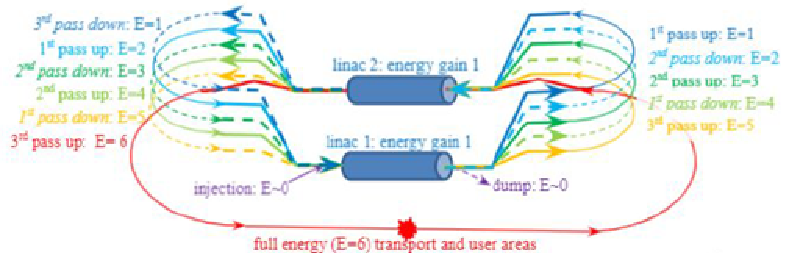
\includegraphics[width=0.8\textwidth]{Figures/DIANA_Inverse_Compton_Source_Design/DIANA_diagram_placeholder.pdf}
\caption{Drawing of the 3-turn DIANA ERL \textcolor{blue}{**PLACEHOLDER**}}
\label{fig:DIANA_ERL_diagram}
\end{figure}
Within the context of the wider accelerator community, this would be a national scale facility and is aligned to two projects in particular: a proposal for the UK-XFEL \cite{burnett2020uk} and as a solution for the Large Hadron--electron Collider (LHeC) \cite{valloni2013strawman,bruning2019exploring,holzer2021accelerator}. Within the wealth of accelerator solutions to a UK x-ray free electron laser presented in the UK-XFEL science case \cite{burnett2020uk}, a partial ERL solution is suggested with an ICS source. The UK-XFEL ICS source work is a precursor to the DIANA ICS source design as DIANA could be a potential demonstrator for the UK-XFEL. In terms of the LHeC project, the DIANA ERL could act as a proof-of-principle for the LHeC ERL alongside the existing PERLE accelerator \cite{angal2018perle}, demonstrating another design and transport approach.

High brilliance electron beams on the \si{\giga\electronvolt}-scale can facilitate applications such as a high power extreme ultraviolet (EUV) FEL and a $\gamma$-ray inverse Compton scattering source. Tunability within the electron bunch energy of the ERL is necessary for many light source experiements and must be central to the design philosophy of DIANA for useful operation of the ICS source and EUV FEL. An EUV FEL source would have far-reaching consequences for semiconductor lithography providing an unparalleled source of 13.5~\si{\nano\meter} EUV radiation (or some harmonic thereof). Whereas a high flux, narrowband  $\gamma$-ray inverse Compton scattering source driven by an ERL would have considerable impact upon nuclear physics and security, beyond the achievements and opportunities available at storage ring facilities such as HI$\gamma$S \cite{weller2009research}. Within the scope of the authors current work, the focus is on the development of the latter application as well a progress toward a conceptual design of the DIANA ERL. Hence, the following chapter excludes EUV FEL developments.

The DIANA ICS source will be driven by the ERL electron bunch, with interaction points designed directly into the transport optics, unlike in the CBETA ICS, to produce a multi-colour $\gamma$-ray source taking advantage of the three nominal energies of the DIANA ERL. A high average power 4-mirror Fabry-Perot optical re-circulation cavity is intended to store the laser pulse and interact this at a high duty factor, producing a high flux and making use of the re-circulated nature of an electron bunch in an ERL. A variable aperture circular collimator placed 10~\si{\meter} from the interaction point will then select the user-desired portion of the spectral output for narrowband operation, making use of the energy--angle correspondence  Through specification of the ERL with a focus toward $\gamma$-ray production and design of the interaction points using optimisation procedures developed in Chapter~\ref{Optimisation_and_Characterisation_of_Inverse_Compton Scattering_Spectra}, the DIANA ICS source aims to produce narrowband ($< 1$\% \textit{rms} BW) radiation on the \si{\mega\electronvolt}-scale. 

A $\gamma$-ray ICS source at moderate energies ($E_{\gamma} < 5$~\si{\mega\electronvolt}) could enable applications such as nuclear resonance fluorescence (NRF) for inspection of nuclear fuel rods, waste studies and detection of clandestine nuclear material \cite{angell2015demonstration,bolind2015states} to high energy ($E_{\gamma} > 5$~\si{\mega\electronvolt}) applications such as nuclear photonics \cite{budker2021expanding} and medical isotope production \cite{habs2011production}. The scattered photon energy regime of nuclear photonics lays in the $\sim$20~\si{\mega\electronvolt} regime and above - at the limitations in energy of the DIANA ICS source. However, the scattered photon energy of the DIANA ICS can be extended to $\sim$40~\si{\mega\electronvolt} through use of frequency doubled lasers such as the commonly used 2nd harmonic of a Nd:YAG ($\lambda =$532~\si{\nano\meter}) laser \cite{} \textcolor{blue}{**WHO SUGGESTS THIS?**}. Within the applications of a DIANA ERL driven ICS source, special consideration is given to the photo-nuclear production of medical isotopes. 

\section{Transport Optics Investigation}
\label{sec:DIANA_transport_optics_investigation}

\section{ERL ICS Electron Beam and Optical Cavity Laser Pulse Parameters}
\subsection{ERL ICS Electron Beam Parameters }
The electron bunch parameters for the DIANA ERL ICS are presented in Table~\ref{tab:DIANA_electron_beam_design_parameters}. The DIANA electron bunch parameters target a high brilliance electron bunch for operation of a high quality ICS and FEL light source facility. The focus of the parameter set displayed here is on maximising the ICS output, however these parameters are broadly applicable to development of a high brilliance FEL, with some adjustment to the longitudinal parameters resulting from the necessity of coherence in FELs requiring short bunch lengths and high peak powers.    

\begin{table}[!h]
\centering
\caption{Electron beam parameters foreseen at the DIANA ICS source interaction point (IP). Baseline parameters assume a round transverse profile for the electron bunch whereas the optimised parameters are the result of a simplex non-round beam optimisation. The given baseline parameters -- which assume the same $\beta^*$ at the IP -- allow a comparison of flux and bandwidth at different energies. The optimised values beneath those are designed to maximise the flux into a 0.5\% \textit{rms} scattered photon bandwidth through a trade-off of $\beta$-function of the electron bunch in each transverse plane and collimation angle.}
\vspace{3mm}
\begin{threeparttable}
\begin{tabular}{lccccc}
\hline\hline
Parameter & \multicolumn{3}{c}{Quantity} & Unit \\
\hline
Turn number & 1 & 2 & 3  \\
Injection Energy, $E_{\mathrm{inj}}$ & \multicolumn{3}{c}{7} & \si{\mega\electronvolt}\\
\tnote{$\dagger$}~Electron kinetic energy, $E_e$ & 362 & 717 & 1072 & \si{\mega\electronvolt}\\
Harmonic Frequency, $f$ & \multicolumn{3}{c}{125} & \si{\mega\hertz}\\
Bunch charge, $e N_e$ & \multicolumn{3}{c}{100} & \si{\pico\coulomb} \\
Avg. beam current, $I$ & \multicolumn{3}{c}{12.5} & \si{\milli\ampere} \\
Transverse normalised \textit{rms} emittance, $\epsilon_{N}$ & \multicolumn{3}{c}{0.5} & \si{\milli\meter}-\si{\milli\radian}\\
\tnote{$\sharp$}~\textit{rms} bunch length, $\Delta \tau$ & \multicolumn{3}{c}{0.9 (3)} & \si{\milli\meter} (\si{\pico\second})\\
Bunch spacing, $t_{b}$ & \multicolumn{3}{c}{8} & \si{\nano\second} \\
RF frequency, $f_{RF}$ & \multicolumn{3}{c}{750} & \si{\mega\hertz} \\
\tnote{*}~Absolute energy spread, $\Delta E_{e}$ & \multicolumn{3}{c}{$\sim$10} & \si{\kilo\electronvolt} \\ 
\tnote{*}~Relative energy spread, $\left(\Delta E_{e}/E_{e}\right)$ & \multicolumn{3}{c}{$\sim10^{-5}$} & \\
\hline
\multicolumn{5}{c}{Baseline Parameters} \\
\hline
$\beta$-functions at the IP, $\beta_{x}^{*}$/$\beta_{y}^{*}$ & 0.2/0.2 & 0.2/0.2 & 0.2/0.2 & \si{\meter} \\
Electron bunch spot size, $\sigma_{e,x}$/$\sigma_{e,y}$ & 11.87/11.87 & 8.44/8.44 & 6.90/6.90 & \si{\micro\meter}\\
\hline\multicolumn{5}{c}{Optimised 0.5\% \textit{rms} Bandwidth} \\
\hline
$\beta$-functions at the IP $\beta_{x}^{*}$/$\beta_{y}^{*}$ & 1.33/0.298 & 2.62/0.587 & 3.90/0.874 & \si{\meter} \\
Electron bunch spot size, $\sigma_{e,x}$/$\sigma_{e,y}$ & 30.62/14.49 & 30.54/14.46 & 30.48/14.43 & \si{\micro\meter}\\
Collimation Angle, $\theta_{\mathrm{col}}$ & 0.180 & 0.091 & 0.061 & \si{\milli\radian} \\ 
\hline\hline
\end{tabular}
\begin{tablenotes}
\item[$\sharp$]{Taken from the ASML FEL parameters \cite{akkermans2017compact}}
\item[*]{Estimated values.}
\item[$\dagger$]{Electron beam energies to accomplish $E_{\gamma}^{\mathrm{max}}$ = 20~\si{\mega\electronvolt} $\gamma$-rays. $\Delta E_{\mathrm{turn}}$ = 355~\si{\mega\electronvolt}.}
\end{tablenotes}
\end{threeparttable}
\label{tab:DIANA_electron_beam_design_parameters}
\end{table}

Baseline parameters are designed in order to maximise the uncollimated flux and brilliance of the ICS source. Therefore, the case of a small interaction point $\beta$-function, which is kept constant, is used to produce a small electron spot size at the IP. The constant $\beta$-function in the baseline case is also useful for highlighting changes within the spectral output that characterises source performance, allowing effects due to the varying kinetic energy of the electron bunch to be disentangled. A non-round beam optimised case is also shown for maximising the collimated flux into a narrow 0.5\% bandwidth, which is optimised using the simplex non-round beam methodology in Chapter~\ref{Optimisation_and_Characterisation_of_Inverse_Compton Scattering_Spectra}. The 0.5\% optimised \textit{rms} bandwidth case is designed to show the ability of DIANA to produce high flux into a narrow bandwidth, required by some nuclear physics experiments, and investigate the difference between ICS source configurations required for both approaches. 

\textcolor{blue}{**JUSTIFY THE PARAMETERS**}
% electron bunch energy
The nominal electron kinetic energies of the DIANA 3-turn ERL are set at 362, 717, 1072~\si{\mega\electronvolt} with a variation in energy per turn of 355~\si{\mega\electronvolt} due to acceleration in the dual linacs from injection of the electron bunch at 7~\si{\mega\electronvolt}. A maximum electron energy of 1072~\si{\mega\electronvolt} is selected as, with a Nd:YAG laser, this allows production of 20~\si{\mega\electronvolt} $\gamma$-rays via inverse Compton scattering which is within the realms of nuclear photonics experiements\cite{} \textcolor{blue}{**NEED SOME REFERENCES**} at the frontier on nuclear physics. The 1072~\si{\mega\electronvolt} maximum energy also reflects the limitations imposed upon the ERL by both physical size and CSR effects. For example, assuming a 20~\si{\mega\volt}/\si{\meter} accelerating electric field \cite{ben2006review}, symmetric linacs and an 80\% filling factor (assumed from CBETA \cite{hoffstaetter2017cbeta}) the length of the linacs would be required to be $\sim$11~\si{\meter}, with the complexities of transport and subsystems this would be an accelerator with $\sim$100's~\si{\meter} circumference. Power loss via CSR would also become a problem at the \si{\giga\electronvolt}-scale, with the limitations of strongly bending arc sections. \textcolor{blue}{**THIS NEEDS SOME WORK**} Because of the maximum electron energy requirements, the nominal energies of the previous turns are fixed at 362~\si{\mega\electronvolt} and 717~\si{\mega\electronvolt}. However, the first turn electron energy is advantageous as this produces scattered photon energies within the energy range for nuclear resonance fluorescence experiments.          

% Injection energy
The injection energy of the DIANA ERL electron bunches is 7~\si{\mega\electronvolt} because this...
\textcolor{blue}{Ask Pete!}

% Harmonic frequency
The bunch repetition frequency of DIANA is set to 125~\si{\mega\hertz}, 1/6th of the RF frequency of the linac at 750~\si{\mega\hertz}, therefore as we have 3-turns only half of the RF buckets are filled. However, we are further bound by the requirement that the laser pulse and electron bunch must interact at the same rate. To satisfy this for a single pulse optical re-circulation cavity and electron bunch must have the same frequency, which means we could operate the laser pulse re-circulation cavity at a maximum bunch rate of 250~\si{\mega\hertz} or any harmonic thereof. It appears that the ideal repetition frequency of both systems is 125~\si{\mega\hertz} driven by the laser pulse optical re-circulation cavity limitations mentioned in the next section. Obviously, the bunch repetition frequency sets the bunch spacing ($t_{b}=1/f$) in the ERL.

% Beam Current (Bunch Charge and REP FREQ dependence)
Average current of the electron bunch in DIANA is 12.5~\si{\milli\ampere}, this is reliant upon the bunch charge and the bunch repetition frequency. Average current is fundamentally limited bu collective effects such as CSR and beam break-up instabilities arising during transport in the ERL, as in CBETA. \textcolor{blue}{Justify 12.5~\si{\milli\ampere}!}

% Transverse Emittance
A small transverse emittance of 0.5~\si{\milli\meter}--\si{\milli\radian} is proposed for the DIANA ERL. Small emittance is necessary for high-brilliance beams and therefore it is a feature of most high brilliance light source projects. Cornell University has previously demonstrated a world-leading transverse emittance of 0.3~\si{\milli\meter}--\si{\milli\radian} from a continuous wave photoinjector \cite{bartnik2015operational}, this photoinjector was applied within the CBETA project, so our specified transverse emittance is well within the state-of-the-art.

% Bunch length
Very short bunch lengths, on a sub-picosecond scale, are possible in the DIANA ERL however this is only desirable in field of ICS sources if the time duration of the radiation is critical for applications. Unlike in FEL applications, where bunch compression would be required for a high peak power electron bunches and to achieve coherent radiation output. Otherwise, the easily attainable picosecond domain is ideal for DIANA as the bunch length of the electron bunch is the same order of magnitude as commercial laser pulse lengths. When the bunch length and the laser pulse length are in the picosecond, domain the reduction in luminosity due to the hourglass effect (Eq.~\ref{eq:furman_hourglass_reduction}) is small, though an angular crossing still results in a modest reduction in flux -- minimising bunch length is a poor way to mitigate this. The value presented for the DIANA ERL is based upon the bunch length within the ASML associated ERL-FEL \cite{akkermans2017compact} with a 3$\sigma$ cut-off, as our discussion of transport options has resulted in the choice of similar optics to this accelerator in a similar electron energy scale.   

% RF Frequency
The RF frequency has been specified at 750~\si{\mega\electronvolt}... \textcolor{blue}{Why?}

% Bunch Energy Spread
A small electron bunch energy spread is necessary for the production of narrowband radiation from both an ICS source and a FEL. The bandwidth of the spectral output of an ICS source is directly proportional to the energy spread of the of the electron bunch. Therefore, it is necessary to minimise the energy spread of the electron bunch for light source operations. The energy spread in Table~\ref{tab:DIANA_electron_beam_design_parameters} is based upon... \textcolor{blue}{**WHERE DOES THIS COME FROM?**}

\subsection{Optical Cavity and Laser Pulse Parameters}

% Why re-circ + Nd:YAG?
The drive laser, a Nd:YAG ($\lambda = 1064$~\si{\nano\meter}) laser, of the inverse Compton scattering source for DIANA is re-circulated, meaning a low pulse energy laser pulse is repetitively interacted within an optical cavity consisting of several high reflectivity mirrors. The re-circulation approach is in contrast to the use of a high power laser, such as a Joule-scale short-pulse Ti:Sa ($\lambda = 800--1100$~\si{\nano\meter}) laser, which has a higher intensity and therefore produced more photons per interaction at the cost of potential non-linear effects. Laser choice must also account for the spectral bandwidth of the laser which is necessary for a narrow bandwidth source, here Nd:YAG lasers typically have smaller spectral bandwidth than Ti:Sa and other high power laser systems. Consequently, for DIANA ICS, the re-circulated approach is selected to avoid non-linear ICS effects such as ponderomotive broadening of the $\gamma$-ray spectral bandwidth, to keep the spectral bandwidth small overall and to take full advantage of the high repetition rate of ERLs, which high powered laser systems can't operate at.      

% 4-mirror + Nd:YAG selection 
Envisioned parameters of the laser pulse provided by a Nd:YAG ($\lambda = 1064$~\si{\nano\meter}) laser and a four mirror Fabry-Perot optical cavity for use in the DIANA ICS source are shown in Table~\ref{tab:DIANA_laser_pulse_design_parameters}. A 4 mirror cavity is selected over a 2 mirror design for improved stability of operation \textcolor{blue}{**WHY IS THIS BETTER?**}. As in the CBETA ICS source (Chapter~\ref{CBETA_Inverse_Compton_Scattering_Source_Design}), an Nd:YAG laser is selected for its picosecond domain and narrow spectral bandwidth. Only a single pulse is recirculated within the optical cavity which is designed to be operated with a fixed \textit{rms} laser pulse waist of radius 25~\si{\micro\meter}. A crossing angle of 5\si{\degree} must be imposed due to the geometry considerations of the 4 mirror cavity.

\begin{table}[!h]
\centering
\caption{Nd:YAG Gaussian laser pulse parameters at the CBETA ICS IP. The interacted laser pulse is produced via a Nd:YAG infrared laser and re-circulated in a bow-tie Fabry-Perot optical cavity.}
\begin{tabular}{lcc}
\hline\hline
Parameter & Quantity & Unit \\
\hline
Wavelength, $\lambda_\textrm{laser}$ & 1064 & \si{\nano\meter}\\
Photon energy, $E_\textrm{laser}$ & 1.17 & \si{\electronvolt}\\
Pulse energy, $E_{pulse}$  & 100 & \si{\micro\joule}\\
Number of photons, $N_{\textrm{laser}}$ & 5.34$\times 10^{14}$ & \\ 
Repetition rate, $f$ & 125 & \si{\mega\hertz}\\
Spot size at the IP, $\sigma_\textrm{laser}$ & 25 & \si{\micro\meter}\\
Crossing angle, $\phi$ & 5 & deg \\
Pulse length, $\tau_{\mathrm{laser}}$  & 10 & \si{\pico\second}\\
Spectral bandwidth (\textit{rms}), $\Delta E_\textrm{laser}/E_\textrm{laser}$ & $\sim10^{-5}$ &   \\
\hline\hline
\end{tabular}
\label{tab:DIANA_laser_pulse_design_parameters}
\end{table}

% Justification of cavity + stored power
These laser pulse parameters are based upon the demonstration of the Fabry-Perot optical cavity in the cERL ICS experiment \cite{akagi2016narrow}. However, they have been modified for a reduced 125~\si{\mega\hertz} repetition rate with an increased pulse energy of 100~\si{\micro\joule} resulting in an increased average stored power of 12.5~\si{\kilo\watt} recirculated in the optical cavity. Therefore, the parameters for the DIANA ICS source are slightly less conservative than those proposed for the CBETA ICS source in Table~\ref{tab:CBETA_laser_pulse_design_parameters} though the MuCLS demonstration of 70~\si{\kilo\watt} \cite{eggl2016munich} affords credibility to these design parameters. The DIANA optical re-circulation cavity also has an  stored power a factor of $\sim50\times$ lower than the state-of-the-art 670~\si{\kilo\watt} average stored power demonstrated by Carstens et al \cite{carstens2014megawatt}, therefore these parameters remain conservative. 

% Justification of rep freq
A repetition frequency of 125~\si{\mega\hertz} results in a cavity path length of 2.4~\si{\meter}, which is tolerable for misalignment errors and within the same scale as the 9.2~\si{\meter} MuCLS optical re-circulation cavity \cite{eggl2016munich}. The laser re-circulation cavity must also remain small so electron bunch focusing optics can achieve a small spot size at the interaction point. Another limitation is mirror heating and damage due to the high peak power per unit area of the laser pulse impinging upon the mirrors within the Fabry-Perot cavity. The peak laser power per unit area upon the cavity mirrors is indirectly related to the repetition frequency as the spot size on the cavity mirrors is related to the path length of the optical cavity and hence the repetition rate.

% Justification of Spot size
A \textit{rms} spot size (radius) on the order of 10's~\si{\micro\meter} is common within ICS sources \cite{} \textcolor{blue}{**COLLECT THESE**}, the waist achieved at cERL ICS (20~\si{\micro\meter}/30~\si{\micro\meter}) \cite{akagi2016narrow} is within the specification here. Using the same laser type (Nd:YAG), with a similar 4 mirror cavity design replication of the cERL ICS laser pulse waist should be possible.


% Justification of crossing angle
A crossing angle is imposed in order to prevent the generated gamma rays from impinging on cavity mirrors and allowing the electron bunch an unobstructed transit through the interaction region. Whilst head-on interactions are possible using strong bending interaction regions that can introduce to the IP and remove the electron bunch within the mirror spacing, as is the case in MuCLS \cite{eggl2016munich}, or via mirrors with holes, which reduces gain in optical re-circulation cavities, these may not be advantageously implemented within ERLs. A crossing angle within a 2--12\si{\degree} range is reasonable, whilst being tolerable for integration of cavity components \cite{variola2011luminosity}. The DIANA ICS uses a 5\si{\degree} crossing angle because the envisioned cavity is based upon the cERL ICS \cite{akagi2016narrow}. 

% Justification of the spectral bandwidth
The spectral bandwidth... \textcolor{blue}{**THIS IS TRICKY**}

\section{ICS Source Spectral Output}

The anticipated spectral output of the DIANA ICS source, using the electron bunch and laser pulse parameters specified in Tables~\ref{tab:DIANA_electron_beam_design_parameters},~\ref{tab:DIANA_laser_pulse_design_parameters}, is presented in Table~\ref{tab:DIANA_spectral_output}. In Table~\ref{tab:DIANA_spectral_output} spectral output parameters are shown for both the 0.5\% \textit{rms} bandwidth optimised case and the baseline case for small electron bunch spot size.

\begin{table}[!h]
\centering
\begin{tabular}{lcccc}
\hline\hline
 & \multicolumn{3}{c}{Electron Kinetic Energy (\si{\mega\electronvolt})} & \\
 \cline{2-4}
 & 362 & 717 & 1072 & \\
\hline
$\gamma$-ray peak energy  & 2.33 & 9.06 & 20.11 & \si{\mega\electronvolt}\\
Source size ($x$/$y$)  & 10.72/10.72 & 8.00/8.00 & 6.65/6.65 & \si{\micro\meter} \\
Uncollimated flux  & 5.77$\times 10^{10}$ & 6.02$\times 10^{10}$ & 6.08$\times 10^{10}$ & ph/\si{\second}\\
Spectral density  & 2.48$\times 10^{5}$ & 6.65$\times 10^{4}$ & 3.03$\times 10^{4}$ & ph/\si{\second} \si{\electronvolt}\\
Average brilliance  & 5.64$\times 10^{12}$ & 2.05$\times 10^{13}$ & 4.45$\times 10^{13}$ & ph/\si{\second} \si{\milli\meter}$^{2}$\si{\milli\radian}$^{2}$ 0.1\% bw\\
Peak brilliance  & 5.60$\times 10^{17}$ & 2.22$\times 10^{18}$ & 4.99$\times 10^{18}$ & ph/\si{\second} \si{\milli\meter}$^{2}$ \si{\milli\radian}$^{2}$ 0.1\% bw\\
\hline
 & \multicolumn{3}{c}{0.5\% \textit{rms} bandwidth} & \\
\hline
Source Size ($x$/$y$) & 19.36/12.54 & 19.35/12.52 & 19.33/12.50 & \si{\micro\meter} \\ 
Collimated flux  & 1.30$\times 10^{9}$ & 1.29$\times 10^{9}$ & 1.29$\times 10^{9}$ & ph/\si{\second} 0.5\% bw \\
\hline\hline
\end{tabular}
\label{tab:DIANA_spectral_output}
\end{table}

% what energies are possible + tunability
Table~\ref{tab:DIANA_spectral_output} shows the DIANA ICS source is capable of producing $\gamma$-rays up to 20.11~\si{\mega\electronvolts}. The first two turns produce 2.33 and 9.06~\si{\mega\electronvolt} $\gamma$-rays however, depending on the tunability of the electron bunch and through variation of the detection angle (due to the energy--angle correspondence), scattered photon energies $< 20.11$~\si{\mega\electronvolt} may be accessible. Tunable $\gamma$-ray energy production will be a focus for future DIANA design work, this is highly dependent on the transport design for the ERL. 

% Why is flux, spec den, avg brill good 
World-class uncollimated flux, spectral density and average brilliance are available from the DIANA ICS source due to the interaction of a high brilliance, high repetition rate electron beam with a high repetition rate re-circulated laser pulse. A comparison of the DIANA ICS source to other designed and operated ICS sources on the \si{\mega\electronvolt}-scale in terms of scattered photon energies and flux is presented in Section~\ref{sec:gamma_ICS_comparison}. The re-circulated nature of this source allows the advantage of high intensity Joule-scale lasers to be overcome delivering a high average power source of $\gamma$-rays. 
\textcolor{blue}{**ADD TO THIS**}

% Why is peak power poor?
Peak power of the DIANA ICS source is reduced in the DIANA ICS source in comparison to other ICS sources \cite{} which typically target $10^{20}$~ph/\si{\second}~\si{\milli\meter}$^{2}$--\si{\milli\radian}$^{2}$~0.1\% BW because the focus of DIANA is producing $\gamma$-rays at a high repetition rate and therefore the focus is on high average brilliance. Modest peak power is due to the low energy of the interacted laser pulse ($E_{\mathrm{pulse}} = 100$~\si{\micro\joule}) and the moderate picosecond durations of the laser pulse and electron bunch. High peak brilliance ICS sources such as \textcolor{blue}{**NAME ONE**} typically target femtosecond electron bunch and laser pulse lengths with Joule-scale laser pulse energies. 

% size at the collimator
At a collimator placed 10~\si{\meter} downstream of the interaction point the spot size (radius) of the produced radiation is of the magnitude $\sim0.1$~\si{\milli\meter}, delivering a pencil beam of $\gamma$-rays for experimental use.

% Bandwidth + minimum theoretical bandwidth
A minimum theoretical bandwidth can be constructed by taking the limit of a small collimation angle ($\theta_{\mathrm{col}}\rightarrow 0$) and large $\beta$-functions ($\beta_{x/y}\rightarrow\infty$) to minimise the emittance (Eq.~\ref{eq:emittance_term}) and collimation (Eq.~\ref{eq:}) terms for the DIANA cases. In reality, these parameters are easily adjustable via the collimator and IP focusing design until they are negligible. Using electron bunch parameters specified in Table~\ref{tab:DIANA_electron_beam_design_parameters} and laser pulse parameters specified in Table~\ref{tab:DIANA_laser_pulse_design_parameters} the minimum theoretical \textit{rms} bandwidth for the DIANA ICS is 0.0022\% i.e 2.2$\times 10^{-5}$. However, due to the assumption of very small laser pulse and energy spreads within this source design, this estimate is likely to be optimistic -- the figures quoted are order of magnitude estimates. 

% Narrowband optimised numbers
The flux around the minimum theoretical bandwidth is also very small, on the order of single photon generations, which is not conducive to experimentation. Typically in ICS sources, the collimation term and emittance term of the bandwidth are dominant when achieving a high flux source. Therefore, to determine a balance betweeen small bandwidth and high flux, it is necessary to select a bandwidth to quantify narrow bandwidth performance. A 0.5\% \textit{rms} bandwidth has been selected because this is within the $<1$\% \textit{rms} bandwidth limit designated as narrow bandwidth within this work, and 0.5\% \texit{rms} BW is of the order of the ELI-NP-GBS $\gamma$-ray source \cite{} \textcolor{blue}{**GET REFERENCES**} (0.5\% \textit{FWHM} BW) which is the current flagship narrowband $\gamma$-ray production facility under construction in Europe. 

The suite of DIANA ICS sources have been optimised for a 0.5\% \textit{rms} bandwidth using the non-round beam simplex optimisation method described in Chapter~\ref{Optimisation_and_Characterisation_of_Inverse_Compton Scattering_Spectra}. The optimised electron beam interaction parameters and collimation parameters shown in Table~\ref{tab:DIANA_electron_beam_design_parameters}. Laser pulse parameters remain unchanged from Table~\ref{tab:DIANA_laser_pulse_design_parameters}. The DIANA ICS source is expected to deliver a collimated flux of 1.30--1.29$\times 10^{9}$~ph/\si{\second} in a 0.5\% \textit{rms} bandwidth, with variation due to the increase in the recoil parameter with electron bunch energy. \textcolor{blue}{**NEED TO PUT THE TABLES IN HERE FOR A COMPARISON OF METHODS**} Furthermore, to characterise narrowband operation of the DIANA ICS sources a series of tuning curves have been devised, based on optimisation methods in Chapter~\ref{Optimisation_and_Characterisation_of_Inverse_Compton Scattering_Spectra}, to show the maximum collimated flux as a function of bandwidth within the narrow bandwidth ($<1$\% \tetxit{rms} BW) regime. 

% Round beam tuning curves
Round-beam tuning curves for the three nominal energies of the DIANA ICS sources (362, 717, 1072~\si{\mega\electronvolt}) are shown in Fig~\ref{fig:DIANA_RB_comparison}, where both the collimated flux--\textit{rms} bandwidth pareto fronts and $\beta$-function at the IP against collimation angle parameter space pareto fronts are shown.  
\begin{figure}[!h]
\centering
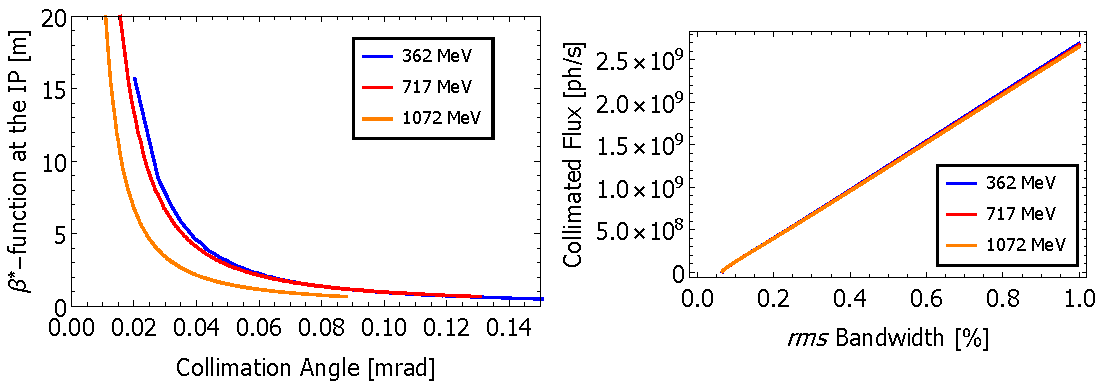
\includegraphics[width=\textwidth]{Figures/DIANA_Inverse_Compton_Source_Design/DIANA_Tuning_Curve_Opt/DIANARBplot.pdf}
\caption{Round beam optimisation comparison at the three nominal energies 362~\si{\mega\electronvolt} (blue), 717~\si{\mega\electronvolt} (red), 1072~\si{\mega\electronvolt} (orange) of the DIANA ICS source. Left: Optimised tuning curves of the $\beta^{*}$-function at the IP (same in both planes) against the collimation angle for each nominal electron energy. Right: collimated flux as a function of the \textit{rms} bandwidth of the DIANA ICS source at each nominal energy.}
\label{fig:DIANA_RB_comparison}
\end{figure}

The $\beta$-function at the IP--collimation angle parameter space tuning curves for each nominal energy in Fig~\ref{fig:DIANA_RB_comparison} each show an 'elbow' style shape, the left hand side of this plot (smaller collimation angle, larger $\beta$-function) corresponds to the narrowest bandwidth therefore smaller flux whereas the right hand side of the plot (larger collimation angle, smaller $\beta$-function) coincides with the highest flux, largest bandwidth optimisations. A difference in energy is observed between the three parameter space tuning curves in the $\beta^{*}$--$\theta_{\mathrm{col}}$ parameter which largely can be explained by the variation in $\psi=\gamma\theta_{\mathrm{col}}$ parameter that appears in the bandwidth, when $\beta^{*}$--$\psi$ is plotted there is a greater agreement between the tuning curves though remaining differences can be explained via the recoil parameter. Within the $\beta^{*}$--$\theta_{\mathrm{col}}$ tuning curve, all configurations above the line are possible with optimised configurations, in the range 0--1\% \textit{rms} bandwidth, laying on the tuning curve.   

The right hand plot of Fig~\ref{fig:DIANA_RB_comparison} shows the pareto front of the collimated flux against the \textit{rms} bandwidth according to the round beam optimisation method. The tuning curve shows the maximum collimated flux available to users within the narrowband regime when the $\beta$-functions in each plane are symmetric. We see only a small variation in the tuning curves due to electron bunch energy which is a reflection of the small variation in the magnitude of the recoil parameter between energies, for example the recoil parameters are $X_{1072~\mathrm{\si{\mega\electronvolt}}} = 0.019$ and $X_{717~\mathrm{\si{\mega\electronvolt}}} = 0.013$ for the DIANA 1072~\si{\mega\electronvolt} and 717~\si{\mega\electronvolt} cases respectively. 

Extension of this optimisation strategy to encompass non-round beam optimisations (see Chapter~\ref{Optimisation_and_Characterisation_of_Inverse_Compton Scattering_Spectra}) has been applied to design of the DIANA interaction points. Tuning curves produces via the three optimisation methods are compared for the DIANA 362~\si{\mega\electronvolt} nominal energy ICS source in Fig~\ref{fig:DIANA362_comparison_optimisation}.

\begin{figure}[!h]
\centering
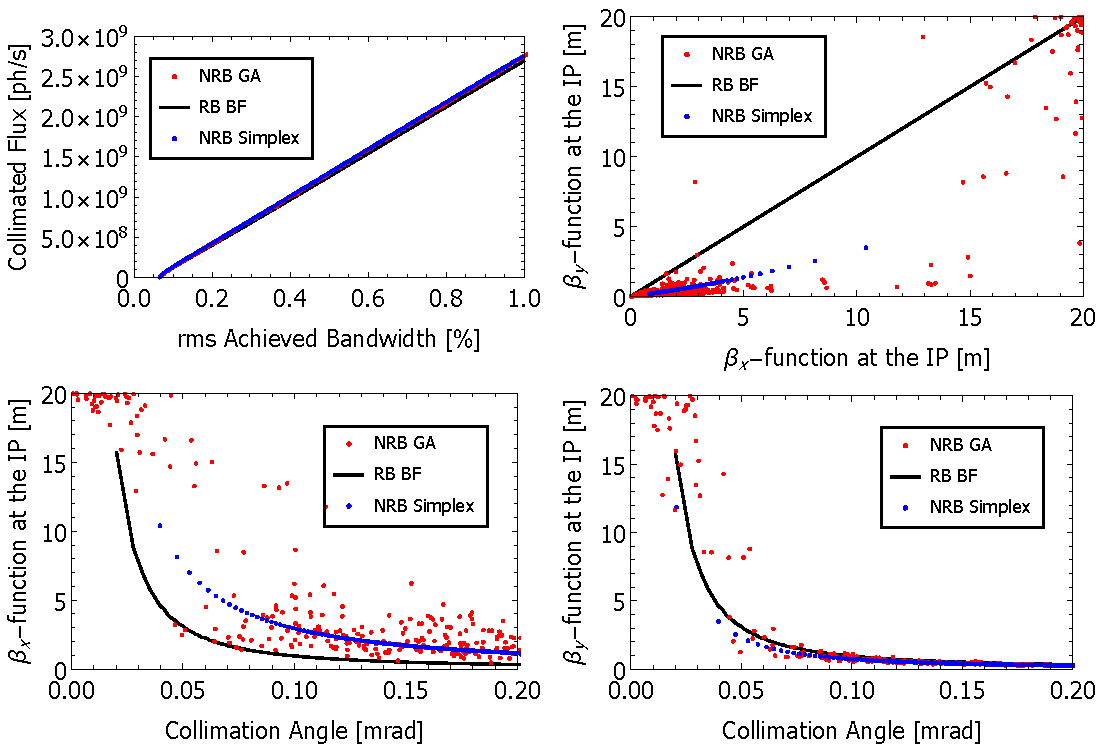
\includegraphics[width=\textwidth]{Figures/DIANA_Inverse_Compton_Source_Design/DIANA_Tuning_Curve_Opt/DIANA362fullcomp.pdf}
\caption{DIANA 362~\si{\mega\electronvolt} 1st turn ICS source optimisations, comparing the two non-round beam approaches (simplex (blue) and GA (red)) and the round beam approach (black). Top Left: collimated flux as a function of \textit{rms} bandwidth pareto fronts of the source. Top Right: interaction point $\beta$-function parameter space in the $x$ and $y$ plane for optimised cases. Bottom Left: parameter space of the interaction $\beta$-function in the $x$ plane and collimation angle for optimised cases. Bottom Right: parameter space of the interaction $\beta$-function in the $y$ plane and collimation angle for optimised cases.}
\label{fig:DIANA362_comparison_optimisation}
\end{figure}

Within Fig~\ref{fig:DIANA362_comparison_optimisation} it is evident that the Pareto front of the collimated flux--\textit{rms} bandwidth is in good agreement between the simplex and genetic algorithm methods. We see that up to $\sim$2.7$\times 10^{9}$~ph/\si{\second} can be produced by DIANA in a narrow bandwidth ($<1$\%). The non-round beam methodologies also produce higher flux within the \textit{rms} bandwidth, than the non-round beam methodology, though both have the same minimum achievable bandwidth. The case of an ERL is a poor case to demonstrate the advantage of a non-round beam optimisation for an ICS IP as the round beam case holds well here, though the increase in flux due to useage of non-round beams is more pronounced at higher $\sim1$\%-scale \textit{rms} bandwidths. 

Plots of the selected $\beta$-functions at the IP in each plane parameter space points corresponding to the Pareto front points in the collimated flux--\textit{rms} bandwidth space in Fig~\ref{fig:DIANA362_comparison_optimisation} show that, as the transverse emittance is identical in each plane, the optimal solution in the easily identifiable simplex case for the IP configuration is to have a larger electron bunch spot size in the $x$-plane than the $y$-plane. Solutions for the $\beta$-functions in each plane clearly diverge from the linear relationship for the round beam case, however the genetic algorithm points are clearly quite polarised to high $\beta$-functions in each plane or low $\beta$-functions in each plane. \textcolor{blue}{**why?**} 

The bottom plots in Fig~\ref{fig:DIANA362_comparison_optimisation} show the $\beta$-functions at the IP in each plane against the required collimation angle for each of the three optimisation methods under consideration. The $\beta_{x}^{*}$--$\theta_{\mathrm{col}}$ plot shows that the non-round beam optimisations maintain the 'elbow' shape as evident in the non-round beam case, however the simplex optimisation is notably offset from the round beam solution. The genetic algorithm $\beta_{x}^{*}$--$\theta_{\mathrm{col}}$ parameter space shows a large stratification of optimal configurations in this plot which highlights the weak dependence on both bandwidth and collimated flux of the $\beta_{x}^{*}$ parameter. However, the $\beta_{y}^{*}$--$\theta_{\mathrm{col}}$ plot shows less stratification for the $\beta_{y}^{*}$ parameter and this also adheres closer to the round beam solution for both the genetic algorithm and simplex cases. Therefore, we can conclude that the variation of the non-round beam in comparison to the round beam case observed in the electron bunch transverse size $x$-plane must be due to the angular crossing, which is the only difference between the two planes.   

Optimisation methods have also been similarly applied to the DIANA 717~\si{\mega\electronvolt} nominal energy ICS interaction. Comparison of these methods and the produced tuning curves for the accelerator are presented in Fig~\ref{fig:DIANA717_comparison_optimisation}.

\begin{figure}[!h]
\centering
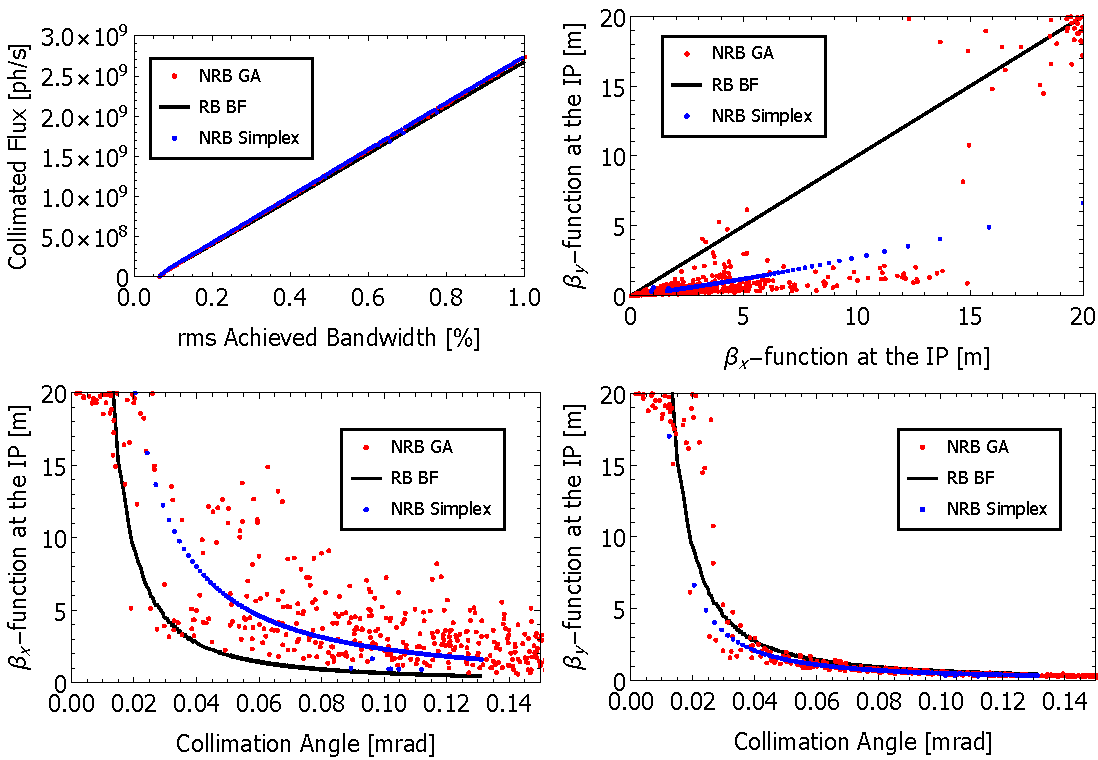
\includegraphics[width=\textwidth]{Figures/DIANA_Inverse_Compton_Source_Design/DIANA_Tuning_Curve_Opt/DIANA717fullcomp.pdf}
\caption{DIANA 717~\si{\mega\electronvolt} 2nd turn ICS source optimisations, comparing the two non-round beam approaches (simplex (blue) and GA (red)) and the round beam approach (black). Top Left: collimated flux as a function of \textit{rms} bandwidth pareto fronts of the source. Top Right: interaction point $\beta$-function parameter space in the $x$ and $y$ plane for optimised cases. Bottom Left: parameter space of the interaction $\beta$-function in the $x$ plane and collimation angle for optimised cases. Bottom Right: parameter space of the interaction $\beta$-function in the $y$ plane and collimation angle for optimised cases.}
\label{fig:DIANA717_comparison_optimisation}
\end{figure}

The solution space and parameter space plots in Fig~\ref{fig:DIANA717_comparison_optimisation} for the ICS source at the 717~\si{\mega\electronvolt} nominal energy appear to show a similar result to the lower energy 362~\si{\mega\electronvolt} nominal energy ICS optimisation. Variation in the Pareto front of the collimated flux against \textit{rms} bandwidth is due to the small increase in the recoil parameter at the higher energy. As noted in the discussion between different nominal electron bunch energy ICS sources in the round beam approach, as shown in Fig~\ref{fig:DIANA_RB_comparison}, the collimation angle appears to vary due to the energy dependence of $\psi = \gamma\theta_{\mathrm{col}}$, however here we also note some variation in the size of the $\beta$-functions at the IP in each plane. The $\beta$-functions appears to become larger with increasing energy due to the energy dependence of the spot size. As is evident from Table~\ref{tab:DIANA_electron_beam_design_parameters}, the spot sizes in each plane remain virtually unchanged due to electron bunch kinetic energy. Overall, better agreement between the parameter space points in the simplex and genetic algorithm methods appears to be achieved for the 717~\si{\mega\electronvolt} nominal energy ICS source optimisations.

Again, the optimisation methods outlined in Chapter~\ref{Optimisation_and_Characterisation_of_Inverse_Compton Scattering_Spectra} have been applied to the highest nominal energy electron bunch ICS interaction within the DIANA ERL. Resulting tuning curves in collimated flux--\textit{rms} bandwidth space and parameter spaces are shown in Fig~\ref{fig:DIANA1072_comparison_optimisation}.

\begin{figure}[!h]
\centering
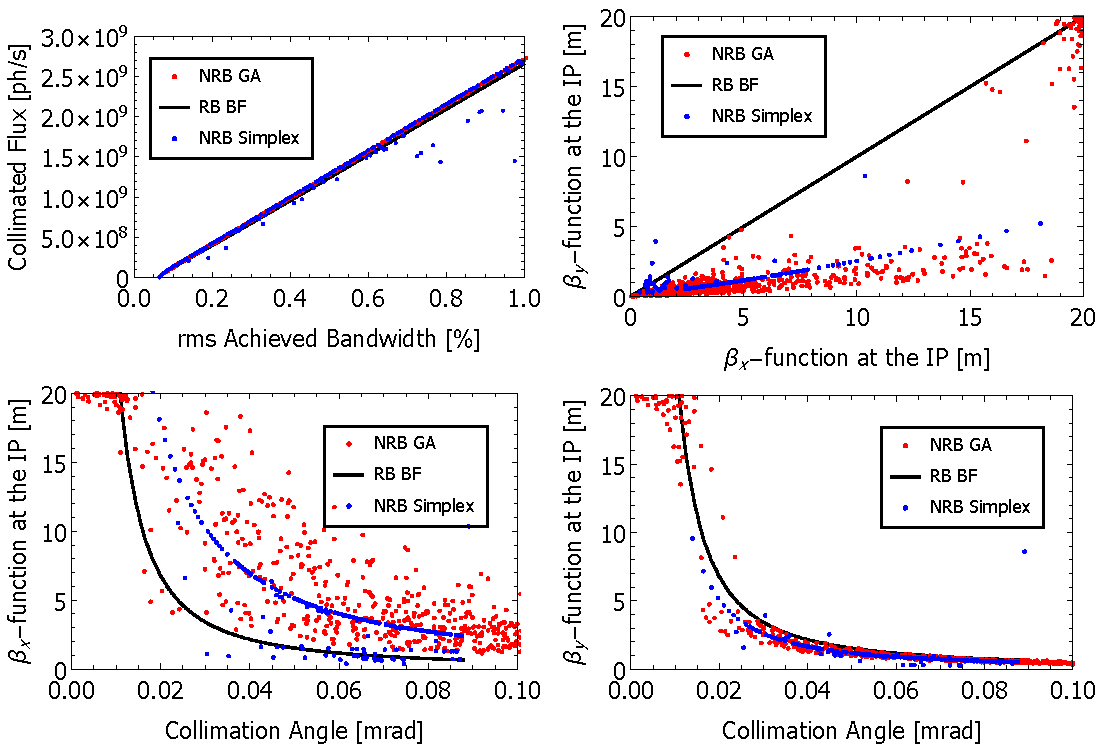
\includegraphics[width=\textwidth]{Figures/DIANA_Inverse_Compton_Source_Design/DIANA_Tuning_Curve_Opt/DIANA1072fullcomp.pdf}
\caption{DIANA 1072~\si{\mega\electronvolt} 3rd turn ICS source optimisations, comparing the two non-round beam approaches (simplex (blue) and GA (red)) with the round beam approach (black). Top Left: collimated flux as a function of \textit{rms} bandwidth pareto fronts of the source. Top Right: interaction point $\beta$-function parameter space in the $x$ and $y$ plane for optimised cases. Bottom Left: parameter space of the interaction $\beta$-function in the $x$ plane and collimation angle for optimised cases. Bottom Right: parameter space of the interaction $\beta$-function in the $y$ plane and collimation angle for optimised cases.}
\label{fig:DIANA1072_comparison_optimisation}
\end{figure}

The suite of optimisations for the 1072~\si{\mega\electronvolt} nominal electron bunch energy, as shown in Fig~\ref{fig:DIANA1072_comparison_optimisation}, are again similar to the optimisations at the two lower nominal electron bunch energies. In the collimated flux--\textit{rms} bandwidth Pareto front, we see more anomalous points which is also visible in the stratification of the simplex points in the parameter space plots. Overall, we see good agreement again between the genetic algorithm method and the simplex method for the 1072~\si{\mega\electronvolt} ICS optimisations. The genetic algorithm results in the $\beta_{x}^{*}$--$\theta_{\mathrm{col}}$ parameter space plot show large variation however, the increase in stratification may be artificial as this effect could be amplified because of the increasing size of the $\beta$-functions in each plane leading to an amplification in the variation between values.    

The performance of a suite of ICS sources driven by the conceptual DIANA 3-turn ERL has been characterised by spectrum plots within a 0.5\% \textit{rms} bandwidth for each nominal energy using the ICARUS code, as described in Chapter~\ref{Optimisation_and_Characterisation_of_Inverse_Compton Scattering_Spectra}. Spectra for ICS sources at 0.5\% \textit{rms} bandwidth are shown in Fig~\ref{fig:}.

\textcolor{blue}{**ICARUS PLOTS FOR DIANA**}

\textcolor{blue}{**describe what these plots mean**}

\section{$\gamma$-ray ICS Source Comparison}
\label{sec:gamma_ICS_comparison}

Inverse Compton scattering sources for production of $\gamma$-rays have been developed and designed worldwide. Differing approaches for the production of $\gamma$-rays have been trialed such as variations on the type of accelerators and incident photon sources used. For example, the HI$\gamma$S source uses radiation produced from a free electron laser to achieve high energy photon production up to 100~\si{\mega\electronvolt}. The most relevant facilities for comparison to the DIANA ICS are tabulated in Table~\ref{tab:gammaray_ICS_comparison}, this presents a combination of operating facilities and recently designed sources. 

\begin{table}[!h]
\caption{Comparison of existing and designed $\gamma$-ray ICS.}
\begin{threeparttable}
\begin{tabular}{lccc}
\hline\hline
ICS & Accelerator Type & Scattered Photon Energy (\si{\mega\electronvolt}) & Flux (ph/\si{\second}) \\
\hline
DIANA\tnote{*} & ERL & 2.33--20.11 & 5.77--6.08$\times 10^{10}$ \\ 
FEBE Exp.\tnote{*} & Linac & $<$1.48 & 4.63--5.83$\times 10^{5} \\
NIJI-IV \cite{sei2017demonstration} & Storage Ring & 1.2 & 3.1$\times 10^{4}$ \\
VIGAS\tnote{*} \cite{shi2021vigas,brenner2020summary} & Linac & 0.2--4.8 & 1--4$\times 10^{8}$ \\
ELI-NP-GBS\tnote{*} \cite{adriani2014technical} & Linac & 0.2--19.5 & $3.9\times 10^{9}$ \\
ELI-NP VEGA\tnote{*} \cite{tanaka2020current,elinp2019vega} & Storage Ring & 1--19.5 & 1$\times 10^{11}$\\
NewSUBARU \cite{utsunomiya2015gamma} & Storage Ring & 5--40 & $3\times 10^{7}$ \\
%VELOCIRAPTOR & Linac & & \\
%T-REX & Linac & & \\
Pan et al CBS\tnote{*} \cite{pan2019design} & Storage Ring & 4--10 & 0.14--3.87$\times 10^{12}$ \\ 
Super-ACO \cite{nutarelli1998gamma} & Storage Ring & 33.4 & $5\times10^{6}$ \\
HI$\gamma$S \cite{weller2009research} & Storage Ring & 1--100 & 5$\times 10^{7}$--5$\times 10^{8}$ \\
\hline\hline
\end{tabular}
\begin{tablenotes}
\item[*]{Denotes design parameters for sources which are not yet demonstrated.}
\end{tablenotes}
\end{threeparttable}
\label{tab:gammaray_ICS_comparison}
\end{table}

% How does DIANA measure up? ENERGY
The DIANA ICS source is designed to produce $\gamma$-rays across a wide  range ($\sim18$~\si{\mega\electronvolt}) of scattered photon energies and will be designed to be steplessly variable within this range via adjustment of the electron bunch energy. The tunability designed for the DIANA ICS matches the tunability of the ELI-NP-VEGA system \cite{tanaka2020current,elinp2019vega}. However, other ICS sources such as NewSUBARU and HI$\gamma$S are capable of producing $\gamma$-rays up to 40~\si{\mega\electronvolt} and 100~\si{\mega\electronvolt} respectively, extending those sources utility into the nuclear photonics regime. High-energy photon capabilites are possible at NewSUBARU and HI$\gamma$S because of two approaches: the use of frequency doubled lasers at short wavelengths, for example a 2nd harmonic Nd:YAG laser ($\lambda = 532$~\si{\nano\meter}) or using short-wavelength radiation from a FEL. The former approach is implementable within the current design of the suite of ICS sources on DIANA yet, to the authors knowledge, high average power short-wavelength optical re-circulation cavities have not been adequately explored. \textcolor{blue}{**True?**}  

% How does DIANA measure up? FLUX
Through examination of Table~\ref{tab:gammaray_ICS_comparison}, it is possible to see that DIANA is of the same order in flux and scattered photon energy as other world-leading source designs such as those by Pan et al and the ELI-NP-VEGA collaboration. A flux of 6.08$\times 10^{11}$ph/\si{\second} is bested by both the Compton Back-scattering Source (CBS) by Pan et al \cite{pan2019design}, which has a factor of 2 larger laser pulse energy, and the ELI-NP-VEGA source, which is also expected to use a higher average stored power cavity, whereas the DIANA ICS source is conservative, and also these assume a head-on interaction, which will be difficult to implement, where in Pan et al \cite{pan2019design} the hourglass effect has been neglected. The hourglass effect would be non-negligible in the Pan et al \cite{pan2019design} CBS case because the electron bunch and laser pulse are both of considerable length ($\sigma_{z,e} = 110$~\si{\milli\meter}, $\sigma_{z,L} = 6$~\si{\milli\meter}) resulting in a luminosity reduction factor of $R_{HG} = $ \textcolor{blue}{**CALCULATE THIS**}. With this in mind, it appears that the DIANA ICS source, the CBS and ELI-NP-VEGA are all capable of similar flux performance. 

% Re-circulation advantage and the abundance of storage ring driven ICS
As is evident from Table~\ref{tab:gammaray_ICS_comparison}, in-depth consideration of an ERL as the driver of an inverse Compton scattering source for production of $\gamma$-rays is limited. Predominantly ICS $\gamma$-ray production is driven by storage ring methods with the existing facilities such as NewSUBARU \cite{utsunomiya2015gamma} and HI$\gamma$S \cite{weller2009research} sources utilising existing synchrotron facilities. World leading facilities such as the ELI-NP $\gamma$-ray source which is currently planned to utilise the Lyncean Technologies variable energy gamma-ray (VEGA) system \cite{tanaka2020current,elinp2019vega} -- a storage ring system, in favour of the ELI-NP-GBS \cite{adriani2014technical}linac system are still therefore based upon the existing storage ring approach. Storage ring sources are undoubtedly favoured because of the high-flux available due to re-circulation of the electron bunch and laser pulse leading to a higher interaction rate. However, as demonstrated in the DIANA ICS source design, because of re-circulation ERL driven ICS sources are capable of high flux operation as in storage ring driven ICS; further evidenced by the similarity in uncollimated flux predicted for DIANA ICS to the flux predictions of leading designs such as ELI-NP VEGA and the CBS \cite{pan2019design} in Table~\ref{tab:gammaray_ICS_comparison}. 

% ERL advantages in bandwidth
Whilst the ERL approach has been shown to be competitive in terms of flux the real advantage of an ERL driven ICS source may be in achieving a narrow bandwidth and production of a large collimated flux per bandwidth. However, quantifying the bandwidth and the collimated flux per bandwidth is difficult as these values are often not quoted within the literature. Narrow bandwidth is necessary for nuclear physics experiments in the $\gamma$-ray regime for example for determining nuclear material composition of mixed isotopic wastes by nuclear resonance fluorescence where isotopic signatures may lie close to one another or for exploiting narrow resonances (Pygmy, Giant Dipole etc.) in nuclear photonics. 

However, storage ring driven ICS sources can suffer from large bandwidth due to large energy spread in the electron bunch, for example with an energy spread of $\sim0.1$\% \cite{litvinenko1996intense}, the minimum possible bandwidth of the HI$\gamma$S ICS source is limited to 0.2\% by this factor alone. In ICS sources the main limitation on the bandwidth is due to emittance and divergence effects, therefore large equilibriated emittances in storage rings such as the large natural emittance ($\epsilon_{x} = 350$~\si{\nano\meter}--\si{radian}) in HI$\gamma$S \cite{weller2009research} lead to large divergence terms in the bandwidth. For example, the large electron bunch energy spread and high emittance of the HI$\gamma$S source limits the produced $\gamma$-ray beam to a 2.5--3.5\% \textit{FWHM} bandwidth \cite{weller2009research} for high flux operation. However, certain storage ring operation modes such as non-equilibrum rings \cite{huang1998laser,owen2013nonequilibrium} and low emittance designs such as the CBS \cite{pan2019design} ($\epsilon_{x} = 8.64$~\si{\nano\meter}--\si{\radian},$\Delta E_{e}/E_{e} = 9.56\times 10^{-4}$) may avoid effects causing poor bandwidth at the cost of a reduction in average electron beam current and subsequently flux.     

Within an ERL both the electron bunch energy spread and large divergence (emittance) limitations are avoided, for example the DIANA ICS source would be capable of a $\sim10^{-5}$ electron bunch energy spread and a small emittance $\epsilon_{nx} = 0.5$~\si{\milli\meter}--\si{\milli\radian} ($\epsilon_{x} = 0.24$~\si{\nano\meter}--\si{\radian}, $E_{e} = 1072$~\si{\mega\electronvolt}), as seen in Table~\ref{tab:DIANA_electron_beam_design_parameters}. Therefore, an ERL driver may be more conducive to design of a high flux, narrowband ICS source than storage rings however specifically designed or operated storage rings potentially could offer similar performance.

\section{Bremsstrahlung Source Comparison}

\textcolor{blue}{**ASK PETE FOR SOUME REFERENCES TO MAKE THE CASE** \\ **HYWEL + PETE SAID NO NEW WORK IS REQUIRED JUST MAKE A CASE**}

\section{DIANA ICS Applications}
% Say only certain examples chosen, not comprehensive

A series of ICS sources driven by the 3-turn ERL DIANA would enable a broad spectrum of experimentation within nuclear photonics \cite{nedorezov2017nuclear} such as nuclear resonance fluorescence and transmutation toward nuclear forensics and security, fundamental nuclear physics, high energy astrophysics, high energy physics and fundamental tests of quantum mechanics as well as medical isotope production. The DIANA ICS source, with spectral output parameters shown in Table~\ref{tab:DIANA_spectral_output}, offers high flux and a narrow bandwidth which are requirements in enhancing experimentation in these areas. The preliminary examination of applications for the DIANA ICS has focused upon nuclear resonance fluorescence and medical isotope production, with potential exploitation of the DIANA ICS source for photonuclear medical isotope production explored in more depth in Section~\ref{sec:photonuclear_medical_isotope_production}.  

% Nuclear Resonance Fluorescence
The first nominal electron kinetic energy ($E_{e} = 362$~\si{\mega\electronvolt}) of the DIANA ICS source is capable of producing tunable $\gamma$-rays with a centroid energy of 2.33~\si{\mega\electronvolt} which is useful for nuclear resonance fluorescence based assays of nuclear materials. Nuclear resonance fluorescence enables isotopic discrimination of materials via resonant absorption of $\gamma$-ray photons at characteristic photon energies then the subsequent emission of $\gamma$-rays at the same energy which is in contrast to XRF -- a suggested application of the CBETA ICS in Chapter~\ref{CBETA_Inverse_Compton_Scattering_Source_Design} -- where a similar process occurs for the atomic levels of atoms allowing elemental discrimination. NRF can be applied to a challenges such as identification of manufacturing defects in fission fuel assemblies, nonproliferation security of spent fission fuel and identification of unknown legacy wastes~\cite{angal2018perle,angell2015demonstration,bolind2015states,geddes2017impact,kwan2011discrete}.

For example, the three isotopes of high importance in nuclear nonproliferation are $^{238}\mathrm{U}$, $^{235}\mathrm{U}$ and $^{239}\mathrm{Pu}$, which display major resonances for incident photon energies of $E_{238~U}^{\mathrm{NRF}} = 2.176$~\si{\mega\electronvolt} \cite{quiter2011transmission},  $E_{235~U}^{\mathrm{NRF}} = 1.733$~\si{\mega\electronvolt} and  $E_{239~Pu}^{\mathrm{NRF}} = 2.143$~\si{\mega\electronvolt} \cite{hayakawa2010nondestructive}, therefore by tuning the electron bunch energy of DIANA in the first pass within the range $E_{\gamma} =$ 312--350~\si{\mega\electronvolt} studies of these isotopes are possible. Resonance spacing between isotopes of interest is often on the order of $\sim10--100$~\si{\kilo\electronvolt}, as evidenced by the difference between $^{238}\mathrm{U}$ and $^{239}\mathrm{Pu}$, therefore narrowband nature and tunability of the bandwidth of the $\gamma$-ray beam is a requirement for isotopic determination by NRF. With a 0.5\% \textit{rms} bandwidth, the first pass ICS source driven by the DIANA ERL has a linewidth of 27.43~\si{\kilo\electronvolt} which is adequate for selective targeting of the nuclear resonances.    

% Transmutation of wastes
Progressing towards the higher energy $\gamma$-rays ($E_{\gamma} =$ 9.06--20.11~\si{\mega\electronvolt}) produced via a DIANA ICS source operating at the 2nd and 3rd turn nominal electron bunch kinetic energy (717, 1072~\si{\mega\electronvolt}) of DIANA, studies such as transmutation of waste and fission dynamics become plausible. Photonuclear transmutation reactions such as $(\gamma,p)$, $(\gamma,n)$, $(\gamma,\alpha)$, $(\gamma,f)$ become possible above 5~\si{\mega\electronvolt} which, when driven by suitable fluxes of photons \textcolor{blue}{**NUMBER?**}, could potentially transform long-lived wastes such as $^{241}\mathrm{Am}$ and $^{129}\mathrm{I}$ into wastes with shorter lifespan or wastes that are easier to handle. 

For example, $^{129}\mathrm{I}$ is a major long lived waste with half-life $T_{1/2} = 1.57\times 10^{8}$~\si{\years}, which poses an additional challenge to repository storage methods \cite{cho2016reconsideration} due to water solubility. Whilst other storage methods are being developed \cite{lee2021chemical,morizet2021immobilization}, another solution would be transmutation of this waste to a stable state, as proposed by Rehman et al \cite{ur2017optimization}, using a giant dipole resonance photonuclear reaction ($\gamma$,n) 
\begin{equation}
^{129}\mathrm{I} \left(T_{1/2}=1.57\times 10^{7}\textrm{y}\right) \xrightarrow[]{\left(\gamma,n\right)} {}^{128}\mathrm{I} \left(T_{1/2}=24.99\mathrm{\si{\minute}}\right) \substack{\xrightarrow[]{\left(\beta^{-},93.1\%\right)} {}^{128}\mathrm{Xe}\left(\mathrm{stable}\right)\\[0.1em] \xrightarrow[]{\left(\beta^{+},6.9\%\right)} {}^{128}\mathrm{Te}\left(\mathrm{stable}\right)}
\label{eq:129I_photonuclear_transmutation}
\end{equation}
where $^{129}\mathrm{I}$ is transmuted to two stable isotopes $^{128}\mathrm{Xe}$ and $^{128}\mathrm{Te}$. Based on the cross section measurements for $^{129}\mathrm{I}$ by J. Magill et al \cite{magill2003laser}, as re-created in Fig~\ref{fig:I129_cross_section_photon_energy} using data from the EXFOR database entry \cite{zerkin2018experimental}, the peak cross section of the photonuclear reaction is $\sigma_{\mathrm{reac}} = 229$~\si{\milli\barn} at 15~\si{\mega\electronvolt}. Tuning DIANA to the required 15~\si{\mega\electronvolt} scattered photon energy would produce a total of $6.04\time 10^{10}$~ph/\si{\second} which, when scaling the transmutation rate with the assumed $10^{13}$~ph/\si{\second} quoted by Rehman et al \cite{ur2017optimization}, would produce a transmutation rate of $\sim10^{8}$~atoms/\si{\second}. Therefore, only miniscule amounts ($\sim0.1$~\si{\micro\gram}) could be processed within a year by this method but there is scope for proof of principle experiments.  

\begin{figure}[!h]
\centering
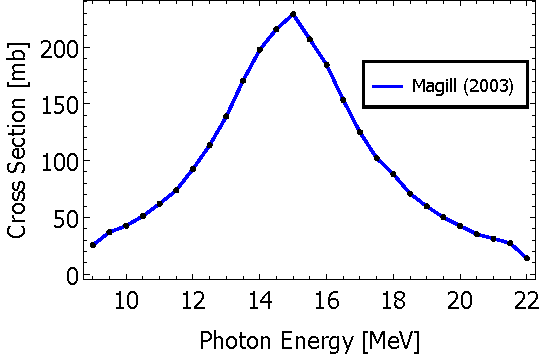
\includegraphics[width=0.7\textwidth]{Figures/DIANA_Inverse_Compton_Source_Design/Iodine_129_cs_photon_energy.pdf}
\caption{Measured \cite{magill2003laser} photonuclear GDR $\left(\gamma,n\right)$ cross section as a function of incident photon energy for the long-lived radioactive waste isotope $^{129}\mathrm{I}$. The cross section peaks at $E_{\gamma} = 15$~\si{\mega\electronvolt} incident photon energy with a cross section of $\sigma = 229$~\si{\milli\barn}. Data acquired from EXFOR database \cite{zerkin2018experimental}.}
\label{fig:I129_cross_section_photon_energy}
\end{figure}

% Fission Dynamics studies
Other experiments of use to the nuclear physics and reactor communities such as fission dynamics studies \cite{bellia1983towards,bhike2017exploratory,finch2018monoenergetic} would also be possible with the suite of DIANA $\gamma$-ray ICS sources. Fission dynamics studies are typically conducted with neutronic probes i.e $\left(n,f\right)$ interactions however there are advantages to conducting these with photofission reactions $\left(\gamma,f\right)$ such as strict angular-momentum selection rules which are well-known, an absence of binding energy in the formation of a compound nucleus and the lack of Coulomb barrier in the interaction due to the neutrality of photons \cite{finch2018monoenergetic}. The photofission GDR reactions of the main isotopes of interest ($^{235}\mathrm{U}$, $^{238}\mathrm{U}$, $^{239}\mathrm{Pu}$) could be investigated from the fission threshold to the high-energy tail of the giant dipole resonance using the DIANA ICS sources, as this requires an energy range $E_{\gamma} =$ 9.0--17.0~\si{\mega\electronvolt} \cite{finch2018monoenergetic}, which is  accessible with steplessly tunable $\gamma$-ray production from the 2nd and 3rd turns ($E_{\gamma} =$ 9.06--20.11~\si{\mega\electronvolt}).

% Fundamental Nuclear Photonics
Collective modes of nuclei such as giant dipole resonances \cite{goldhaber1948nuclear,baldwin1947photo}, pygmy dipole resonances \cite{cook1957photodisintegration,tonchev2010spectral} and scissor modes \cite{de1984reformulation,bohle1984new} can be probed via NRF techniques using $\gamma$-ray ICS sources. For example, the M1 scissors mode of a $^{152}\textrm{Sm}$ nucleus has recently been probed at the HI$\gamma$S source to investigate the electric quadrupole (E2) mode decay \cite{ide20212}. However, this experiment has been limited by the large 100~\si{\kilo\electronvolt} \textit{FWHM} bandwidth \cite{ide20212} of the source at the $E_{\gamma} = 2.995$~\si{\mega\electronvolt} incident $\gamma$-ray energy required to probe the scissor mode \cite{ziegler1993low} and consequently excited states beyond the $2^{+}$ state are inaccessible because of the insensitivity of the incident $\gamma$-ray beam \cite{ide20212}. However, based on the DIANA ERL ICS source calculations at 362~\si{\mega\electronvolt} ($E_{\gamma} =$ 2.33~\si{\mega\electronvolt}) for a 0.5\% \textit{rms} bandwidth the \textit{FWHM} energy spread of the $\gamma$-ray beam is 27.43~\si{\kilo\electronvolt}, a factor $\sim3$ smaller than the HI$\gamma$S bandwidth, which can still be minimised further. The DIANA ICS source is also design to produce comparatively larger flux than HI$\gamma$S, as seen in Table~\ref{tab:gammaray_ICS_comparison}, which will improve data acquisition times for these measurements. Studies such as these are also targeted by the ELIADE research program utilising ELI-NP-VEGA \cite{elinp2019vega}, which concerns high-resolution studies of E1, M1, and E2 modes where the aim is to It will be possible to distinguish and separate different excitations in the overlapping region of the
pygmy dipole resonance (PDR), the giant dipole resonance (GDR), the magnetic dipole resonance (MDR), and the pygmy quadrupole resonance (PQR) \cite{tanaka2020current}.

\section{Photonuclear Medical Isotope Production}
\label{sec:photonuclear_medical_isotope_production}

\textcolor{blue}{**BLURB ABOUT MEDICAL ISOTOPES, TREATMENT, IMAGING, THERANOSTIC etc.**\\**PRODUCTION METHODS - REACTOR, CYCLOTRON**}

Radionuclides have abundant uses within the realms of medical treatment, with application in imaging, such as $\beta^{+}$ emitting isotopes like $^{18}\mathrm{F}$ with wide use from tumour volume imaging studies \cite{rocha2021metabolic} to investigations of long Covid-19 \cite{sollini2021long}, in treatment, such as prostate cancer brachytherapy \cite{yuan2021proof} with $^{192}\textrm{Ir}$ ($T_{1/2} =73.83$~\si{\day}, $\beta^{-}$, 95.13\%, $\epsilon$, 4.87\%). Theranostic \cite{svenson2013theranostics} radionuclide treatments, where isotopes or combinations thereof find use within joint imagining and treatment, have became a recent focus in this area of research. For example, $^{64}\mathrm{Cu}$ is a theranostic isotope which decays through $\beta^{+}$ (61\%) and $\beta^{-}$ (39\%) with the emission of Auger electrons \cite{boschi2018emerging}; allowing simultaneous diagnostic imaging and therapy with the same radio-pharmaceutical.

A range of production methods for medical isotopes are available such as cyclotron based production \cite{} with $\left(p,x\right)$ reactions, research reactor production \cite{} with $\left(n,x\right)$ reactions, isotope separation on-line (ISOL) production with $\left(p,f\right)$ reactions \cite{} as well as the photonuclear production methods with $\left(\gamma,x\right)$ reactions \cite{habs2011production}. \textcolor{blue}{**NO CARRIER ADDED PRODUCTION, WHY ISOL IS GOOD (MASS SPEC), WHY PHOTONUCLEAR IS GOOD (NARROWBAND)}. 

Using the DIANA ICS source, with high flux and narrow bandwidth, preliminary experiments on the photonuclear production of medical isotopes could be undertaken. A series of candidates have been evaluated for production using DIANA, with particular focus on the photoneutron $\left(\gamma,n\right)$ reaction. Within this section photonuclear production of two promising medical isotope candidates: $^{153}\mathrm{Sm}$ and $^{155}\mathrm{Tb}$ will be investigated.  

\subsection{Samarium 153 Production}

Samarium 153 is a well established radionuclide used in the commercial radio-pharmaceuticals Quadramet \cite{ema2015quadramet} -- Samarium lexidronam pentasodium -- which via $\beta^{-}$ decay 
\begin{equation}
^{153}\mathrm{Sm} \left(T_{1/2} = 1.93~\mathrm{\si{\day}}\right)\xrightarrow[]{\left(\beta^{-},\mathrm{100\%}\right)} {}^{153}\mathrm{Eu},
\label{eq:153Sm_beta_minus_decay}    
\end{equation}
is used as a therapy for palliation of bone metastases \cite{kapoor2021cancer,murray2021systemic}. Typically, $^{153}\mathrm{Sm}$ is produced in a research reactor via 
\begin{align}
^{152}\mathrm{Sm}&\xrightarrow[]{\left(n,\gamma\right)}{}^{153}\mathrm{Sm} \\
^{154}\mathrm{Sm}&\xrightarrow[]{\left(n,2n\right)}{}^{153}\mathrm{Sm}
\label{eq:153Sm_research_reactor_production}
\end{align}
neutron capture reactions using highly enriched Samarium targets. Enriched $^{152}\mathrm{Sm}$ and $^{154}\mathrm{Sm}$ targets can be produced using electromagnetic isotope separators which has been demonstrated at Oak Ridge Laboratory using Caultrons producing enrichments of $>$98\% respectively \cite{bell1987stable}. These highly enriched Samarium isotope targets are now available commercially at enrichments of $>$98.4\% and $>$98.5\% \cite{isoflex2021sm}. However, due to the relatively short half-life of $^{153}\mathrm{Sm}$ ($T_{1/2} = 1.93$~\si{\day}) and the neutron rich environment of a reactor, research reactor irradiation production methods are suceptible to contamination with $^{154}\mathrm{Eu}$ \cite{naseri2021effective,van2018separation} via
\begin{equation}
^{153}\mathrm{Sm}\xrightarrow[]{\left(\beta^{-},\mathrm{100\%}\right)}{}^{153}\mathrm{Eu}\xrightarrow[]{\left(n,\gamma\right)}{}^{154}\mathrm{Eu},
\label{eq:153Sm_reactor_contamination}    
\end{equation}
typically occurs where the $^{153}\mathrm{Sm}$ $\beta^{-}$ decays during irradiation to $^{153}\mathrm{Eu}$ which then undergoes neutron capture $\left(n,\gamma\right)$ to $^{154}\mathrm{Eu}$. The $^{154}\mathrm{Eu}$ contaminant is relatively long-lived ($T_{1/2} = 8.59$~y), which results in difficulties for storage and handling of $^{153}\mathrm{Sm}$ based radiopharmaceuticals and a short 24 hour shelf-life \cite{ema2015quadramet} as the prevalence of $^{154}\mathrm{Eu}$ impurities becomes too high \cite{van2018separation}.

However, photonuclear production of $^{153}\mathrm{Sm}$ \cite{carlos1974giant,filipescu2014photoneutron} is possible via
\begin{equation}
^{154}\mathrm{Sm}\xrightarrow[]{\left(\gamma,n\right)}{}^{153}\mathrm{Sm},
\label{eq:153Sm_photonuclear_production}    
\end{equation}
using an ICS $\gamma$-ray source such as DIANA and a highly enriched ($>$98\%) $^{154}\mathrm{Sm}$ target \cite{bell1987stable,isoflex2021sm}. There are several competing photonuclear processes alongside the pathway targeted in (Eq.~\ref{eq:153Sm_photonuclear_production}) such as \cite{carlos1974giant}
\begin{align}
^{154}\mathrm{Sm}\xrightarrow[]{\left(\gamma,2n\right)}{}^{152}\mathrm{Sm},\\
^{154}\mathrm{Sm}\xrightarrow[]{\left(\gamma,n\right)+\left(\gamma,np\right)}{}^{153}\mathrm{Sm}+{}^{152}\mathrm{Pm},
\label{eq:153Sm_photonuclear_disruptors}    
\end{align}
for a mono-isotopic $^{154}\mathrm{Sm}$ target. More competing processes may occur, such as a $\left(\gamma,3n\right)$ reaction etc. however data for these is unavailable in the EXFOR database \cite{zerkin2018experimental} and the literature, we limit this discussion to the measured cross-sections. A full study of impurities would be required, but this is beyond the scope of this investigation.   The cross section of the desired (Eq.~\ref{eq:153Sm_photonuclear_production}) and measured disruptive (Eq.~\ref{eq:153Sm_photonuclear_disruptors}) photonuclear processes as a function of $\gamma$-ray photon energy in Fig.~\ref{fig:154Sm_cross_section_photon_energy}.

\begin{figure}[!h]
\centering
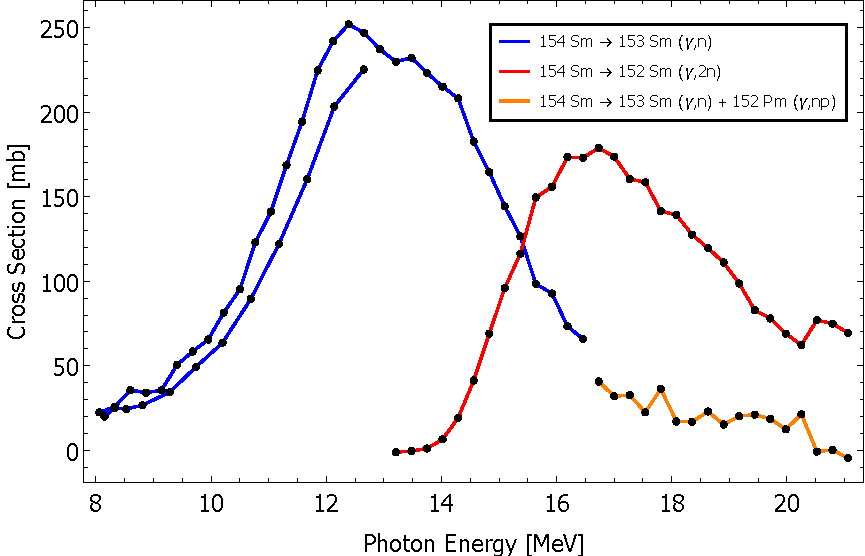
\includegraphics[width=0.8\textwidth]{Figures/DIANA_Inverse_Compton_Source_Design/Sm154Landscape.pdf}
\caption{Reaction cross section against incident photon energy for the $^{154}\mathrm{Sm} \left(\gamma,n\right)$ reaction of interest (blue, higher data \cite{carlos1974giant}, lower data \cite{filipescu2014photoneutron}), and the potentially disruptive reactions $^{154}\mathrm{Sm} \left(\gamma,2n\right)$ (red \cite{carlos1974giant}) and $^{154}\mathrm{Sm} \left(\gamma,n\right) + \left(\gamma,np\right)$ (orange \cite{carlos1974giant}). Data for other reactions photonuclear reactions involving $^{154}\mathrm{Sm}$ was unavailable. Data acquired from the EXFOR database \cite{zerkin2018experimental}. }
\label{fig:154Sm_cross_section_photon_energy}
\end{figure}

In Fig.~\ref{fig:}, two measurements of the $^{154}\mathrm{Sm}\left(\gamma,n\right)$ cross section are made by Filipescu et al \cite{filipescu2014photoneutron} using the NewSUBARU $\gamma$-ray source \cite{utsunomiya2015gamma} and Carlos et al \cite{carlos1974giant} where monochromatic $\gamma$-rays were generated using in-flight positron annihilation \cite{miller1960monochromatic}, where a positron beam impinges upon a target, in a 60~\si{\mega\electronvolt} linac at Saclay \cite{audit1970etude}. In-flight positron annihilation methods produce both a narrowband radiation spectral line resulting from positron--electron the annihilations in the target as well as the typical Bremsstrahlung radiation spectrum; the two can't be disentangled, but the ratio of the signal of the positron annihilation to the Bremsstrahlung spectrum can typically be maximised through use of a small collimation angle resulting in collimated fluxes of $1.5\times10^{3}$~ph/\si{\second} and \textit{FWHM} bandwidths of $\sim 12$\% for the upgraded Saclay source \cite{veyssiere1979quasi}. Comparing the Saclay positron source with the NewSUBARU ICS source in Table~\ref{tab:gammaray_ICS_comparison} and using the approximation $\mathcal{F}_{\mathrm{0.1\%}} = 1.5\times 10^{-3}\mathcal{F}$ \cite{krafft2010compton}, the flux for the NewSUBARU ICS source would be higher than the upgraded Saclay positron annihilation source \cite{veyssiere1979quasi} therefore this measurement has a better signal to noise ratio and the \textit{FWHM} bandwidth of NewSUBARU is 1-2\%, a factor of 6 improvement on the Saclaay upgraded source. Therefore, the NewSUBARU $^{153}\mathrm{Sm}\left(\gamma,n\right)$ measurement offers superior precision. 


Fig.~\ref{fig:154Sm_cross_section_photon_energy} shows that the known competing processes for a mono-isotopic $^{154}\mathrm{Sm}$ can be avoided below 13.21~\si{\mega\electronvolt} as this is the threshold for the $^{154}\mathrm{Sm}\left(\gamma,2n\right)$ photonuclear reaction. However, some of the data presented by Carlos et al \cite{carlos1974giant} for the disruptive processes has negative cross sections, which appears to be unphysical. The peak cross sections for the desired $^{154}\mathrm{Sm}\left(\gamma,n\right)$ reaction are $\sigma_{\mathrm{reac}} = 252.1$~\si{\milli\barn} at $E_{\gamma} = 12.39$~\si{\mega\electronvolt} (Carlos et al \cite{carlos1974giant}) and $\sigma_{\mathrm{reac}} = 225.3$~\si{\milli\barn} at $E_{\gamma} = 12.65$~\si{\mega\electronvolt} (Filipescu et al \cite{filipescu2014photoneutron}). Therefore, with the DIANA ICS source tuned to the scattered photon energy corresponding to the peak cross section, photonuclear production of $^{153}\mathrm{Sm}$ is possible.

The specific activity of a radioisotope produced using a photonuclear method can be calculated simply based on the assumption that we produce a pure radioisotope without admixture of stable isotopes \cite{habs2011production} and we assume that other photoneutron reations, for example a $\left(\gamma,n\right)$ reaction on a produced radisotope, do not interfere during irradiation. The resultant specific activity ($A/m$) in \si{\becquerel}/\si{\milli\gram} of a produced radioisotope at irradiation time $t_{\mathrm{irr}}$ is given by \cite{habs2011production}
\begin{equation}
\frac{A}{m} = \frac{N_{A}}{M}\sigma_{\mathrm{reac}}\Phi\left\{1-\exp\left[\frac{-\ln\left(2\right)t_{\mathrm{irr}}}{T_{1/2}}\right]\right\},
\label{eq:specific_activity}    
\end{equation}
where $N_{A}$ is Avogadros constant, $M$ is the molar mass of the target isotope, $\sigma_{\mathrm{reac}}$ is the cross section of the reaction used to generate the radionuclide and $T_{1/2}$ is the half-life of the generated radioisotope and $\Phi$ is the flux density in ph/(\si{\second}~$\mathrm{\si{\milli\meter}}^2$) at the target. The flux density at the target is calculated by the collimated flux in a 0.5\% bandwidth at the scattered photon energy corresponding to the peak cross section, either through scaling or re-optimisation, and the area on the target is calculated assuming a circular collimator and no divergence of the produced $\gamma$-ray beam, which produces a circular spot on the target. We have also assumed that all of the 0.5\% \textit{rms} bandwidth acts at the peak cross section, which is an overestimation. 

At saturation, where sufficiently long irradiation time overcomes the half-life the specific activity becomes maximal
\begin{equation}
\left(\frac{A}{m}\right)_{\mathrm{max}} = \frac{N_{A}}{M}\sigma_{\mathrm{reac}}\Phi.
\label{eq:sat_specific_activity}    
\end{equation}
To get an order of magnitude estimate for the specific activity for the photonuclear production of $^{153}\mathrm{Sm}$ using DIANA, the assumption that the collimated flux in a 0.5\% \textit{rms} bandwidth ($\mathcal{F} = 1.30\times 10^{9}$~ph/\si{\second}) is concentrated at the peak photonuclear cross section is made. The peak cross section assumption results in a slight overestimation of the produced specific activity, however optimisation of the bandwidth and accounting for the full energy dependence of the cross section for photonuclear production of radioisotopes is beyond the scope of this work. The specific activity as a function of irradiation time for $^{153}\mathrm{Sm}$ is shown in Fig.~\ref{fig:153Sm_specific_activity}.
\begin{figure}[!h]
\centering
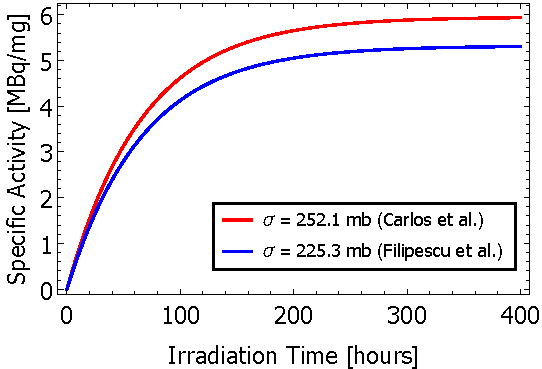
\includegraphics[width=0.6\textwidth]{Figures/DIANA_Inverse_Compton_Source_Design/154Sm_specific_activity.pdf}
\caption{Estimated specific activity of the produced $^{153}\mathrm{Sm}$ as a function of irradiation time using the collimated flux of the DIANA ICS source operating in a 0.5\% \textit{rms} bandwidth at the peak photoneutron reaction cross section, as measured by Carlos et al \cite{carlos1974giant} (red) and Filipescu et al \cite{filipescu2014photoneutron} (blue).}
\label{fig:153Sm_specific_activity}
\end{figure}

As shown in Fig.~\ref{fig:153Sm_specific_activity}, within around 10 days of irradiation the specific activity of the sample reaches a maximum of 66.92~\si{\mega\becquerel}/\si{\milli\gram} (Carlos et al \cite{carlos1974giant}) and 61.07~\si{\mega\becquerel}/\si{\milli\gram} (Filipescu et al \cite{filipescu2014photoneutron}). However, if there are irradiation time constraints, as is likely, the radioisotopic sample will not achieve the saturated specific activity. 

Typically, Quadramet is produced for clinical applications with a specific activity of 16--65~\si{\mega\becquerel}/\si{\micro\gram} \cite{ema2015quadramet}, a factor of $\sim$1000 below the current estimate for the photoneutron route. Therefore, photonuclear production of $^{153}\mathrm{Sm}$ is currently below viable commercial production standards because of the low reaction cross section, flux limitations of the DIANA ICS source and a lack of optimisation of this method. With optical cavities on the 100's~\si{\kilo\watt} scale becoming widely available \cite{eggl2016munich,liu2018optical}, the possibility of improving interaction dynamics using crab cavities \cite{variola2011luminosity,koshiba2018luminosity} and the increasing the average power frontier of ERLs, photonuclear production of radioisotopes could become plausible. There is also the additional possibility of increasing specific activity by targeting nuclear resonances for improved photoneutron reaction cross sections \cite{habs2011production}, though this hasn't been investigated within this work. However, proof-of-principle experiments involving photoneutron production of $^{153}\mathrm{Sm}$ could be conducted at the DIANA $\gamma$-ray ICS source, and optimisation of photonuclear production of radioisotopes is a possible topic for future work.      

\subsection{Terbium 155 Production}
% 155 Tb
Isotopes of Terbium, specifically the Terbium radioisotope quadruplet \cite{muller2012unique}, are highly regarded as a candidate for theranostic use where the four clinically useful candidates are: $^{149}\mathrm{Tb}$, $^{152}\mathrm{Tb}$, $^{155}\mathrm{Tb}$ and $^{161}\mathrm{Tb}$. The lowest mass isotope $^{149}\mathrm{Tb}$ ($T_{1/2} = 4.12$~\si{\hour}) decays via $\alpha$ emission, which could have many applications in oncology \cite{muller2017alpha} including treatment of leukemia and lymphoma \cite{beyer2004targeted}. The highest mass isotope $^{161}\mathrm{Tb}$ ($T_{1/2} = 6.89$~\si{\day}) decays exclusively via a low-energy $\beta^{-}$ decay route producing Auger electrons \cite{muller2012unique}, which is being explored at the trial phase as a treatment for prostate cancer \cite{baum2021first,muller2019terbium} and may be advantageous over $^{177}\mathrm{Lu}$ ($T_{1/2} = $~\si{}) to which $^{161}\mathrm{Tb}$ has similar decay characteristics with the production of more Auger electrons \cite{lehenberger2011low,grunberg2014anti}. Both $^{152}\mathrm{Tb}$ and $^{155}\mathrm{Tb}$ are useful in imaging; $^{152}\mathrm{Tb}$ decays via $\beta^{+}$ decay and therefore is useful in PET imaging \cite{muller2012unique}, whereas $^{155}\mathrm{Tb}$ ($T_{1/2} = 5.32$~\si{\day}) decays exclusively by electron capture and could be used in SPECT imaging to provide tumour imaging without a high radiation dose burden to the patient \cite{muller2012unique}.

These isotopes are typically produced using spallation methods; $^{161}\mathrm{Tb}$ is produced using neutron spallation of highly enriched $^{160}\mathrm{Gd}$ targets \cite{lehenberger2011low} whereas the other three isotopes have all been produced via high energy ($E_{e} = 1.4$~\si{\giga\electronvolt}) proton spallation \cite{muller2012unique} at the CERN-MEDICIS facility \cite{dos2014cern} with isotope separation on-line (ISOL) at the ISOLDE \cite{catherall2017isolde} facility. Deutron spallation techniques have also been used for the production of $^{155}\mathrm{Tb}$ using 34~\si{\mega\electronvolt} deutrons from the ARRONAX cyclotron \cite{duchemin2016deuteron}. 

Spallation methods with ISOL are typically expensive and complex facilities \cite{duchemin2016deuteron}, with only a handful worldwide such as the SPES-ISOLPHARM experiment \cite{andrighetto2019isolpharm} and no existing dedicated production facilities based on this method. The spallation and ISOL method consequently focuses on isotopes that are difficult to produce via more conventional research reactor and cyclotron based approaches. Therefore, an opportunity exists to develop alternative methods to produce isotopes solely available at ISOL facilities without the cost and complexity of high energy spallation and isotope separation on-line. The photonuclear route could provide some of these isotopes with less complexity; here we present a case study for one such isotope -- $^{155}\mathrm{Tb}$.

Terbium 155 is useful in SPECT imaging via the electron capture decay
\begin{equation}
^{155}\mathrm{Tb}\left(T_{1/2} = 5.32~\mathrm{\si{\day}}\right)\xrightarrow[]{\left(\mathrm{EC}, \mathrm{100\%}\right)}{}^{155}\mathrm{Gd},
\label{eq:Tb155_decay}
\end{equation}
which produces $\gamma$-rays at 86.55~\si{\kilo\electronvolt} (32\%) and 105.3~\si{\kilo\electronvolt} (25\%)\cite{muller2012unique} which are useful for SPECT imaging. A possible photonuclear route to produce $^{155}\mathrm{Tb}$ is via a photoneutron reaction $\left(\gamma,n\right)$ and subsequent exclusive $\beta^{+}$ decay from $^{156}\mathrm{Dy}$
\begin{equation}
^{156}\mathrm{Dy}\xrightarrow[]{\left(\gamma,n\right)}{}^{155}\mathrm{Dy}\left(T_{1/2} = 9.92~\mathrm{\si{\hour}}\right)\xrightarrow[]{\left(\beta^{+},\mathrm{100\%}\right)}{}^{155}\mathrm{Tb}.    
\label{eq:155Tb_photonuclear_production}
\end{equation}
Production via this route (Eq.~\ref{eq:155Tb_photonuclear_production}) would require a monoisotopic target of $^{156}\mathrm{Dy}$, however 156 Dysprosium isotope has a particularly low abunance in natural Dysprosium (0.056\%) and therefore requires enrichment. Enrichment via electromagnetic isotope separators, such as Caultrons \cite{bell1987stable}, can provide $< 34\%$ pure $^{156}\mathrm{Dy}$ whilst commercially $^{156}\mathrm{Dy}$ is available at $< 20.7\%$ enrichment \cite{}. Improvement in enrichment may be possible using lasers with methods such as separation of isotopes by laser excitation (SILEX)\cite{} \textcolor{blue}{**SILEX explanation, some examples ETC**} Because enrichment is so low for commercially available target isotopes, unlike in the $^{153}\mathrm{Sm}$ case, we must account for photoneutron reactions from other isotopes of Dysprosium in the assesment of the cross section.

The $^{156}\mathrm{Dy}\left(\gamma,n\right){}^{155}\mathrm{Dy}$ photoneutron reaction has a small cross section ($\sigma_{\mathrm{reac}} = 144\pm 44$~\si{\milli\barn}) \cite{vagena2017photodisintegration}, measured as an average cross section across a wide range of energies using a Bremsstrahlung method driven by an electron linac and tungsten target. However, several competing reactions to the $^{156}\mathrm{Dy}\left(\gamma,n\right){}^{155}\mathrm{Dy}$ reaction exist such as \cite{renstrom2018verification,vagena2017photodisintegration}
\begin{align}
^{163}\mathrm{Dy}&\xrightarrow[]{\left(\gamma,n\right)}{}^{162}\mathrm{Dy}, \\
^{162}\mathrm{Dy}&\xrightarrow[]{\left(\gamma,n\right)}{}^{161}\mathrm{Dy}, \\
^{158}\mathrm{Dy}&\xrightarrow[]{\left(\gamma,n\right)}{}^{157}\mathrm{Dy}, \\
^{156}\mathrm{Dy}&\xrightarrow[]{\left(\gamma,n\right)}{}^{155}\mathrm{Dy},
\label{eq:155Tb_photonuclear_disruptors}    
\end{align}
where higher order ($\gamma,2n$ etc.) reactions and those involving protons or alpha particles have no known measurement \cite{zerkin2018experimental}.

The photoneutron reaction cross sections as a function of incident photon energy are shown in Fig.~\ref{fig:}
\begin{figure}[!h]
\centering
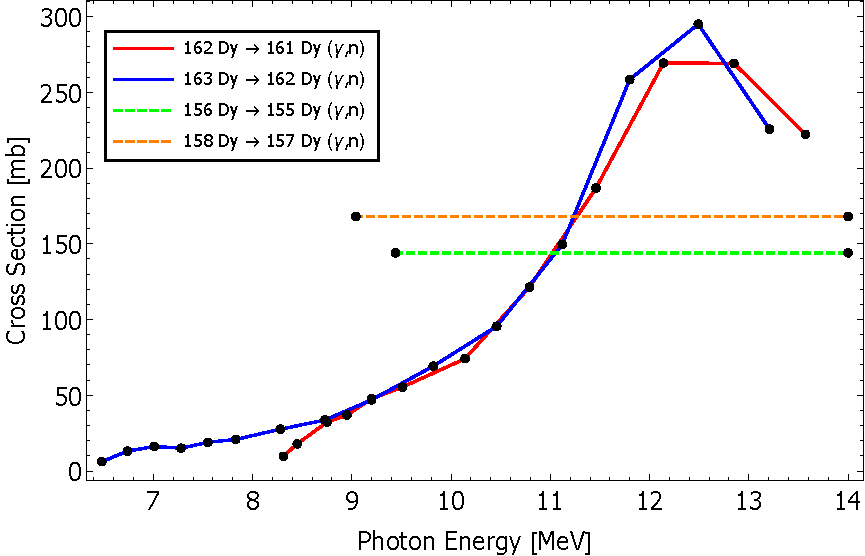
\includegraphics[width=0.8\textwidth]{Figures/DIANA_Inverse_Compton_Source_Design/DyLandscape.pdf}
\caption{Reaction cross section as a function of incident photon energy for measured photoneutron reactions from $^{\mathrm{nat}}\mathrm{Dy}$ including the desired $^{156}\mathrm{Dy}\left(\gamma,n\right){}^{155}\mathrm{Dy}$ (green \cite{vagena2017photodisintegration}) reaction and the disruptors $^{163}\mathrm{Dy}\left(\gamma,n\right){}^{162}\mathrm{Dy}$ (blue \cite{renstrom2018verification}), $^{162}\mathrm{Dy}\left(\gamma,n\right){}^{161}\mathrm{Dy}$ (red \cite{renstrom2018verification}) and $^{158}\mathrm{Dy}\left(\gamma,n\right){}^{157}\mathrm{Dy}$ (orange \cite{vagena2017photodisintegration}). Data for other $^{\mathrm{nat}}\mathrm{nat}$ reactions is unavailable. Dashed lines represent average cross section measurements \cite{vagena2017photodisintegration}, whereas full lines are cross section measurements made at varied incident photon energies. The EXFOR database has been used as a source of these measurements \cite{zerkin2018experimental}. }
\label{fig:Dy_cross_section_energy)}
\end{figure}

Fig.~\ref{fig:Dy_cross_section_energy)} shows that it will be difficult to produce no carrier added $^{155}\mathrm{Tb}$ from $^{\mathrm{nat}}\mathrm{Dy}$ as the competing reactions overlap in incident photon energy. Therefore, highly enriched dysprosium targets or chemical separation \cite{webster2019chemical}, which is also required in the spallation and ISOL approach, are necessary to production of high radioisotopic purity samples. The cross section measured by Vagena and Stoulos for the $^{156}\mathrm{Dy}\left(\gamma,n\right){}^{155}\mathrm{Dy}$ photoneutron reaction is $\sigma_{\mathrm{reac}} = 144\pm 44$~\si{\milli\barn}, which has a large error bar due to the nature of the Bremsstrahlung measurement method which has used integrated flux  within a large energy range defined by the reaction threshold and the maximum possible energy of the Bremsstrahlung source limited by the electron bunch energy of the linac. In contrast, precise measurements of the $^{162}\mathrm{Dy}\left(\gamma,n\right)$ and $^{163}\mathrm{Dy}\left(\gamma,n\right)$ reactions where narrower band photon spectra are used as the experimental probe \cite{renstrom2018verification}.

An order of magnitude estimate of the specific activity possible from  photoneutron production of $^{155}\mathrm{Dy}$ is possible using the collimated flux in a 0.5\% \textit{rms}  bandwidth of the DIANA ICS source, where we assume that the reaction cross section is constant at its peak value. This allows for an order of magnitude estimate of the specific activity of the $^{155}\mathrm{Tb}$ radioisotope which, as it has a longer half-life ($T_{1/2} = 5.32$~\si{\day}) than the intermediary $^{155}\mathrm{Dy}$ ($\left(T_{1/2} = 9.92\right)$~\si{\hour}), is the remaining isotope after a long irradiation. \textcolor{blue}{**THIS FEELS WOOLY, SURELY A MATHEMATICAL WAY TO DO THIS**} The measurement by Vagena and Stoulos \cite{vagena2017photodisintegration} is an average photoneutron reaction cross section within a photon energy range, therefore in order to correctly calculate the specific activity we make the assumption that the incident photon energy from DIANA, which we assume is steplessly variable, lies at the midpoint of this range $E_{\gamma} = 11.52$~\si{\mega\electronvolt}. Specific activity as a function of irradiation time is shown for the shorter-lived $^{155}\mathrm{Dy}$ intermediary in Fig.~\ref{fig:155Dy_specific_activity} with the 1$\sigma$ maximum and minimum cross section variation cases also plotted.
\begin{figure}[!h]
\centering
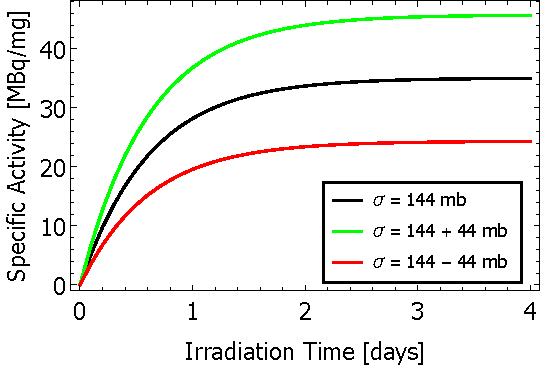
\includegraphics[width=0.6\textwidth]{Figures/DIANA_Inverse_Compton_Source_Design/155Dy_specific_activity.pdf}
\caption{Estimated specific activity of the produced $^{155}\mathrm{Dy}$ as a function of irradiation time using the collimated flux of the DIANA ICS source in a 0.5\% \textit{rms} bandwidth around a centroid scattered photon energy of $E_{\gamma} = 11.52$~\si{\mega\electronvolt}, the midpoint of the energy range measured by Vagena and Stoulos \cite{vagena2017photodisintegration} in the average reaction cross section measurement ($\sigma_{\mathrm{reac}} = 144$~\si{\milli\barn}) (black) and for values with $1\sigma$ error: $\sigma_{\mathrm{reac}} = 144 + 44$~\si{\milli\barn} (green) and $\sigma_{\mathrm{reac}} = 144 - 44$~\si{\milli\barn} (red).} 
\label{fig:155Dy_specific_activity}
\end{figure}
As shown in Fig.~\ref{fig:155Dy_specific_activity}, the specific activity of $^{155}\mathrm{Dy}$ saturates at $35.06\pm 10.71$~\si{\mega\becquerel}/\si{\milli\gram}, which occurs within a resonable $\sim$3 day duration. Assuming the same specific activity for the $^{155}\mathrm{Tb}$ radioisotope, the photoneutron production of $^{155}\mathrm{Tb}$ can be compared to spallation and ISOL methods via conversion of the specific activity to the widely used clinical units of
\si{\mega\becquerel}/\si{\nano\mole}. The CERN-MEDICIS facility have produced $^{155}\mathrm{Tb}$-cm09 at a specific activity of 0.64~\si{\mega\becquerel}/\si{\nano\mole} \cite{muller2012unique} whereas in the photoneutron production study here the specific activity is 5.43~\si{\kilo\becquerel}/\si{\nano\mole}, a factor of 117 below the spallation and ISOL method. However, the laser parameters in Table~\ref{tab:DIANA_laser_pulse_design_parameters} for the DIANA ICS source are conservative, the photonuetron production has not been optimised -- a standard 0.5\% \textit{rms} bandwidth collimated flux is used -- and the measurement of the cross section is just an average cross section, which is an underestimate as a narrowband $\gamma$-ray ICS source is capable of targeting resonance peaks. Hence, the estimated 5.43~\si{\kilo\becquerel}/\si{\nano\mole} specific activity of $^{155}\mathrm{Tb}$ shows promise for photonuclear production of $^{155}\mathrm{Tb}$.

In summary, production of $^{155}\mathrm{Tb}$ via the DIANA ICS source appears to be feasible and is a candiate for proof of principle medical isotope production using a DIANA ICS source. However, challenges to the photonuclear production of $^{155}\mathrm{Tb}$ exist, such as the enrichment of $^{156}\mathrm{Dy}$ targets and the requirement of improved measurement of the $^{156}\mathrm{Dy}\left(\gamma,n\right)$ cross section. At $\sim20$\% enrichment, $^{156}\mathrm{Dy}$ targets make production of no carrier added $^{155}\mathrm{Dy}$ difficult, though methods such as SILEX \cite{} may improve enrichment and chemical separation techniques \cite{webster2019chemical} can ameliorate this issue by removing impurities in the radioisotopic sample. The measurement of the $^{156}\mathrm{Dy}\left(\gamma,n\right)$ cross section is not fit for purpose, though it could be improved by measurement with ICS source, for example the higher quality measurements of $^{163}\mathrm{Dy}\left(\gamma,n\right)$ and $^{162}\mathrm{Dy}\left(\gamma,n\right)$ using the HI$\gamma$S ICS source \cite{renstrom2018verification}. Measuring photoneutron reaction cross sections could be a major application of the DIANA ICS source because DIANA can produce narrower band radiation than HI$\gamma$S, the leading $\gamma$-ray source, and also operates at a comparatively higher flux. These challenges are additional to the flux limitations and that are explored for the $^{153}\mathrm{Sm}$ photonuclear production case, therefore production of $^{155}\mathrm{Tb}$ is more complex.  

\section{Summary}

\end{document}